\chapter{Introduction}

\section{CERN and the LHC}

The European Organization for Nuclear Research, or CERN, is an international institution tasked with providing particle accelerators to scientists for purposes of conducting high energy physics experiments. It is the home of the LHC (Large Hadron Collider) accelerator chain, comprised primarily of LINAC4, the PS (Proton Synchrotron), the PSB (Proton Synchrotron Booster), the SPS (Super Proton Synchrotron) and the LHC itself, a particle accelerator with circumference of 27 kilometers around. It is located across the Franco-Swiss border local to Lake Geneva, the Jura mountains, and Mont Salève.

\begin{figure}
    \centering
    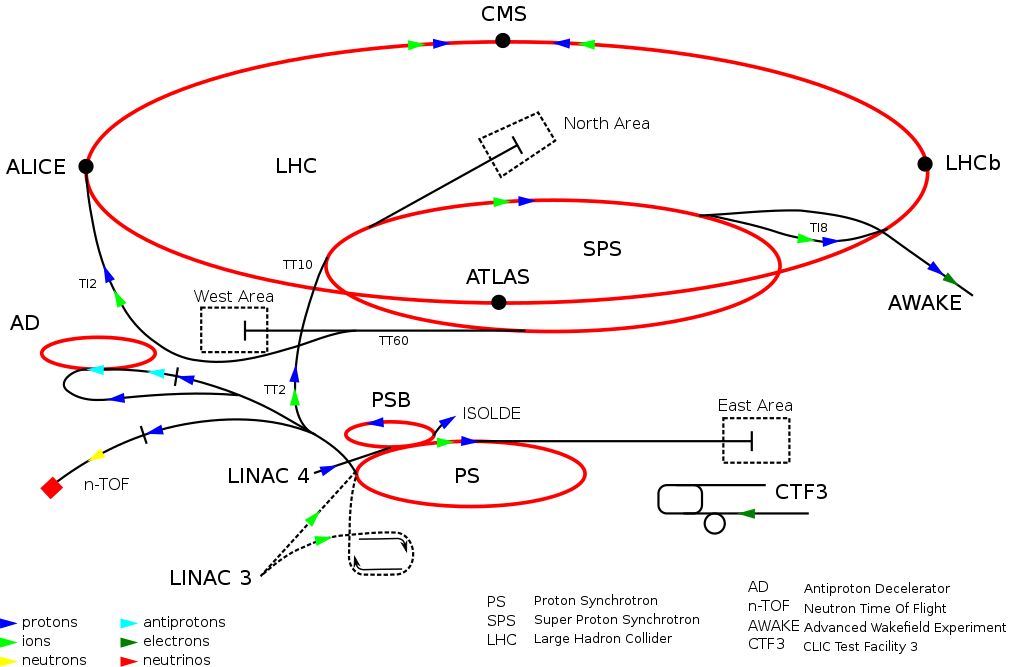
\includegraphics{figs/1024px-Cern-accelerator-complex.svg.png}
    \caption{The CERN Accelerator Complex includes various particle injectors such as the PS and SPS, and large detection experiments such as ATLAS and CMS \cite{forthomme_cern_2021}.}
    \label{fig:cern}
\end{figure}

The LHC collides energetic and intense proton bunches against one other so that the resulting particles produced in these collisions can be observed and analyzed. Upon analysis, these observations may provide evidence for particle's predicted to exist according to the Standard Model of particle physics, namely the Higgs Boson. These particle's may vary in charge, spin, mass, momentum, etc. Often weakly interacting with matter, so their qualities must be quantified through the use of large particle detector systems. For example, the CMS (Compact Muon Solenoid) experiment is comprised of solenoids to probe a particle's momentum from perceived magnetic rigidity, calorimeters to estimate particle energy deposition, and micro-channel plates to qualify time-of-flight and generalized position tracking measurements, as depicted in Figure~\ref{fig:cms}.

\begin{figure}
    \centering
    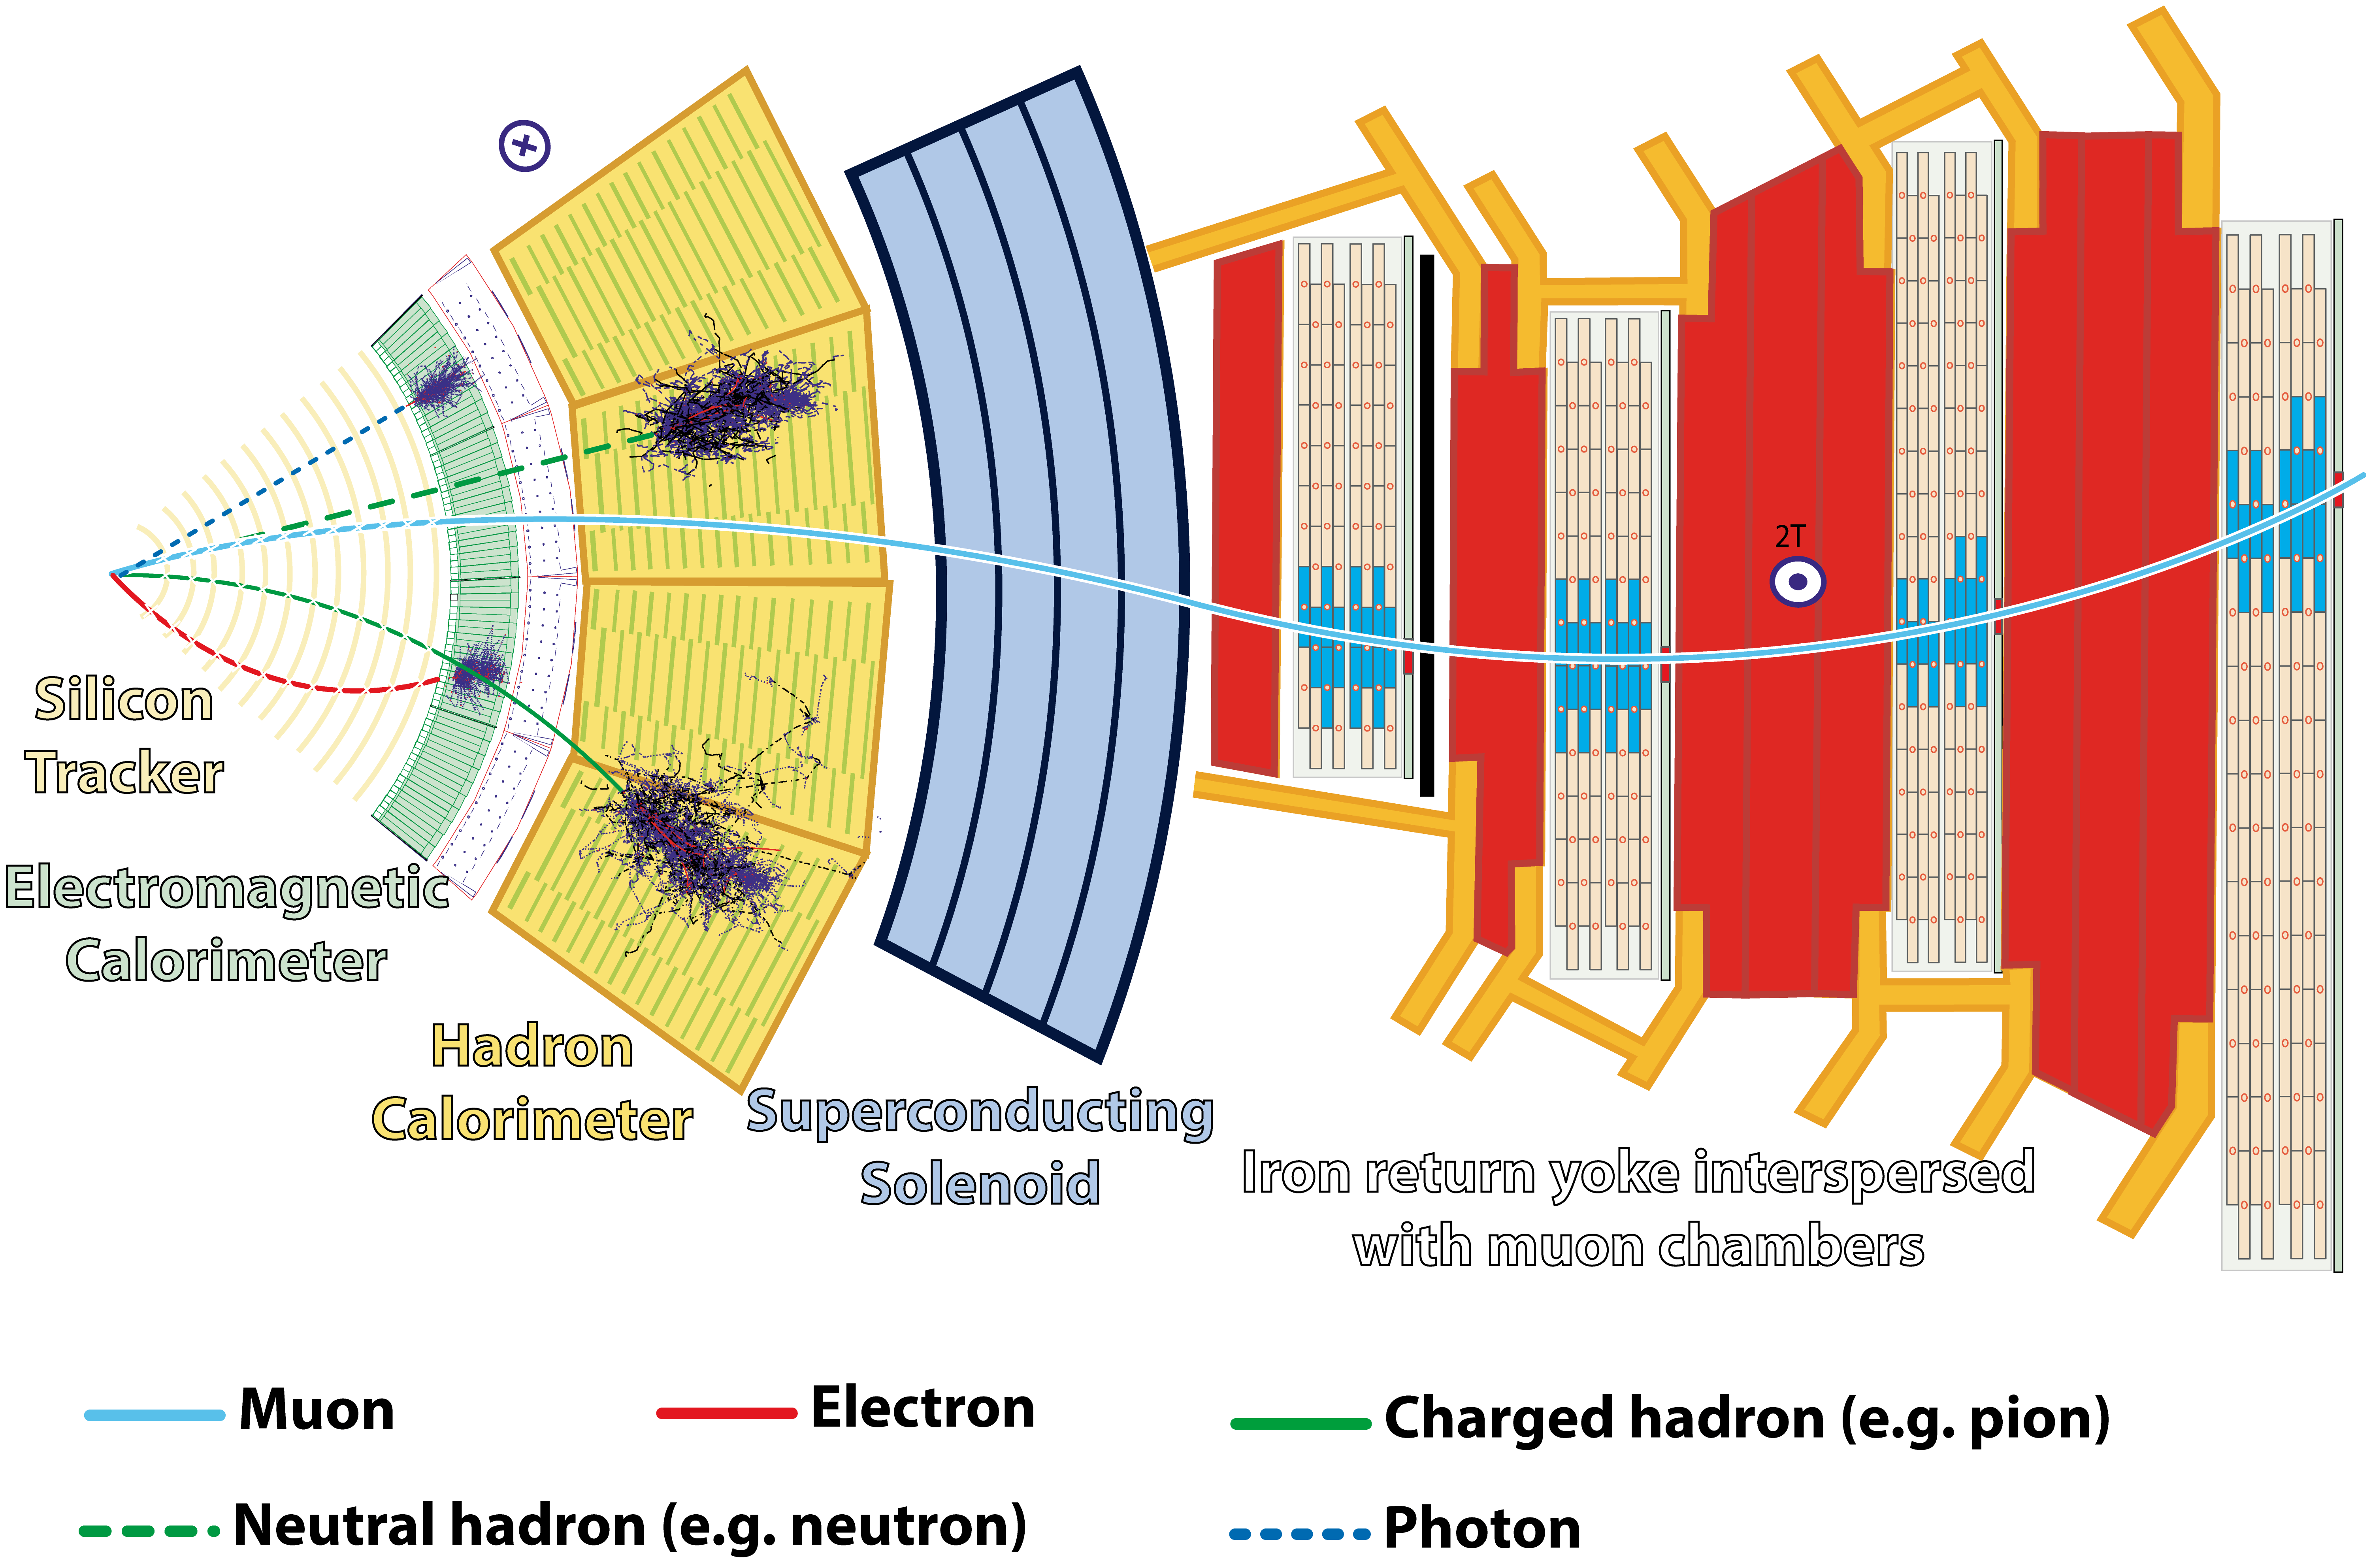
\includegraphics{figs/CMSslice_whiteBackground.png}
    \caption{Particles generated by proton-proton collisions within the LHC Radial pursue radial trajectories through the CMS detector \cite{barney_cms_2016}.}
    \label{fig:cms}
\end{figure}

To verify the existence of the Higgs Boson, physicists must be able to resolve the energy spectra corresponding to the various particles produced in proton-proton collisions. To mitigate large experimental uncertainty due to collision variance and the particle product variability, the total number of interaction \textit{events} must be increased. This can be done by increasing the interaction luminosity along with total acquisition time. We see in \eqref{eq:luminosity} how, for a bivariate gaussian beam, the luminosity ($\mathcal{L}$) scales with number of bunches $n_B$, particles per bunch $N$ and inversely with beam width $\sigma$ per

\begin{equation}
    \mathcal{L} = \frac{n_b N^2f_{rep}}{4\pi\sigma_x\sigma_y}H_d
    \label{eq:luminosity}.
\end{equation}

Because acquisition time is already a strong limitation, there is an ever persistent effort to improve the beam luminosity, effectively defined by the quality of the injectors. This is the motivation behind the HL-LHC (High Luminosity LHC) initiative whose goal is to increase beam luminosity by a factor of 10 \cite{aberle_high-luminosity_2020}. The LIU (LHC Injectors Upgrade) project is directed to upgrading the injectors to deliver the required additional beam brightness \cite{damerau_lhc_2014}.

\section{Space-Charge Limitations}

As particle beam intensities are increased to improve luminosity, the electromagnetic fields of charged particle bunches will self-interact. This interaction, named \textit{space-charge}, may cause the bunch to repel apart, break up, or induce other instabilities and perturbations yielding to overall transmission loss. In the transverse plane, maintaining a tight beam size is accomplished through the use of strong focusing optics and by reaching higher beam energies whereas in the longitudinal plane, space-charge becomes critical during injection and extraction where the efficiency of transferring bunches from one ring to the next is highly dependent on how short the bunch length can be kept. Instabilities that can lengthen the bunch length can therefore negatively impact total beam brightness factored towards the LHC.

As will be discussed further in the text, a particle within a bunch will experience a longitudinal \textit{induced voltage} $$\Delta V = \frac{-i}{\omega_s}\frac{Z}{n}\frac{d\lambda}{d\tau}$$ dependent on the \textit{longitudinal space-charge impedance} given by $$\frac{Z}{n} = -i\frac{Z_0}{\beta\gamma^2}g$$ which scales inversely with $\beta \gamma^2$. Accordingly, induced voltage due to space-charge is generally a low energy effect except at the highest bunch intensities.

Small perturbations and density fluctuations in the bunch's longitudinal charge density profile can create self amplifying wakefield fluctuations that can lead to \textit{micro-bunch instabilities}. As observed in Figure~\ref{fig:microbunch_instabilities}, a narrow bunch distribution can spontaneously split due to local fluctuations in the bunch profile that have a negative feedback mechanism for promoting further instabilities.

\begin{figure}
    \centering
    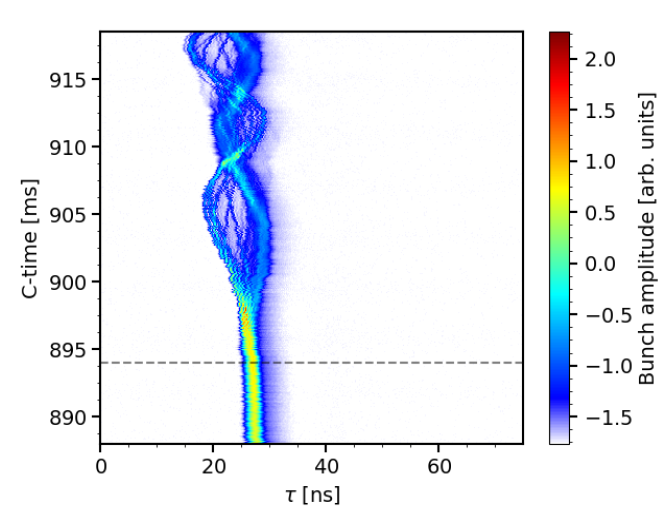
\includegraphics{figs/micro_bunching_instabilities.PNG}
    \caption{Example of micro-bunch instabilities simulated in the longitudinal tracking code BLond. Small fluctuations in the longitudinal profile induce wakefield modulations which self-influence the bunch, inducing beam breakup.}
    \label{fig:microbunch_instabilities}
\end{figure}

\section{Particle Injectors}

In the PS (Proton Synchrotron), the particle energy is accelerated from 2-26 GeV in 3.6 seconds (Table~\ref{tab:ps_parameters}). Accordingly where space-charge is an important consideration towards the beginning of its ramp, at relativistic energies, the PS can neglect space-charge towards extraction.

\begin{table}
    \centering
    \begin{tabular}{lccc}
        Parameter                  & Symbol        & Injection                      & Extraction \\
        \hline
        Circumference (m)          & C             & \multicolumn{2}{c}{628}                     \\
        Kinetic Energy (GeV)       & W             & 1.4                            & 25         \\
        Lorentz Factor             & $\gamma$      & 2.5                            & 27.7       \\
        Revolution Frequency (kHz) & $f_s$         & 436                            & 476        \\
        RF Harmonic                & $h$           & 7                              & 21         \\
        RF Frequency (MHz)         & $f_{RF}$      & 3                              & 10         \\
        Synchrotron Frequency (Hz) & $\Omega_s$    & 600                            & 230        \\
        Synchrotron Tune           & $Q_s$         & 0.00137                        & 0.00048    \\
        Transverse Tune            & $Q_x, Q_y$    & \multicolumn{2}{c}{6.21, 6.24}              \\
        Transition Factor          & $\gamma_t$    & 6.1                            & 6.1        \\
        Bunch Width (ns)           & $\sigma_\tau$ & 26                             & 1
    \end{tabular}
    \caption{Injection/Extraction parameters for PS at flat-top"' and 'flat-bottom' respectively.}
    \label{tab:ps_parameters}
\end{table}

As seen in Figure~\ref{fig:ps_impedance}, the space-charge impedance is nearly compensated by the ring's effective inductive impedance near transition energies at which point the synchronism between RF systems, magnetic field ramp, and bunch phase, requires dynamic adjustment to maintain longitudinal stability. Accordingly there is a lot of potential for space-charge induced instabilities to degrade the bunch during ramp and therefore is of particular interest for space-charge studies.

\begin{figure}
    \centering
    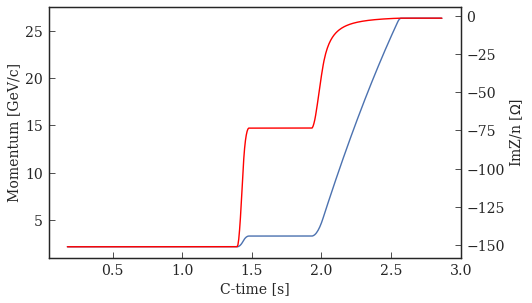
\includegraphics{figs/energy_v_space_charge_impedance.png}
    \caption{Proton momentum (blue) compared with red (inductive impedance) during PS Ramp \cite{lasheen_alexandre_ps_2020}.}
    \label{fig:ps_impedance}
\end{figure}

The luminosity of proton-proton collisions occurring within the LHC is almost strictly defined by the beam intensity achieved from the injector chain. At low energies and high intensities, as in LINAC4 and the PS, space-charge effects are fighting to destabilize the beam, hence motivation to raise the injection energy in the PS.

\section{RF Manipulations in the PS}

Protons are injected into the PS from the four superimposed rings of the PSB (Proton Synchrotron Booster) as depicted in Figure~\ref{fig:ps_complex}.

\begin{figure}
    \centering
    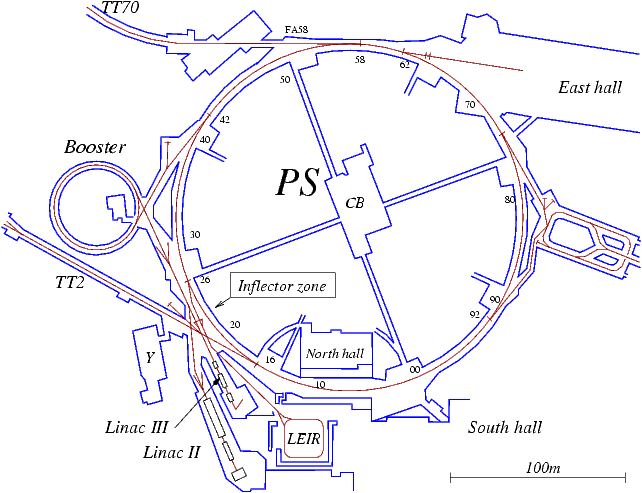
\includegraphics{figs/pscomplex.png}
    \caption{The PS complex \cite{belleman_ps_2020}, LINAC4 replacing LINAC2 (not pictured) as the start of the LHC injector chain.}
    \label{fig:ps_complex}
\end{figure}

At these lower energies, space-charge dominates and accordingly particle energies must be increased before bunches can be merged. As observed in Figure~\ref{fig:bcms}, the PS conducts a series of \textit{manipulations} where RF voltage profiles of varying harmonics are used to position, accelerate, merge and then split the bunches longitudinally according to the varying space-charge limitations. This BCMS (batch compression matching and splitting) process is visualized in Figure~\ref{fig:bcms}.

\begin{figure}
    \centering
    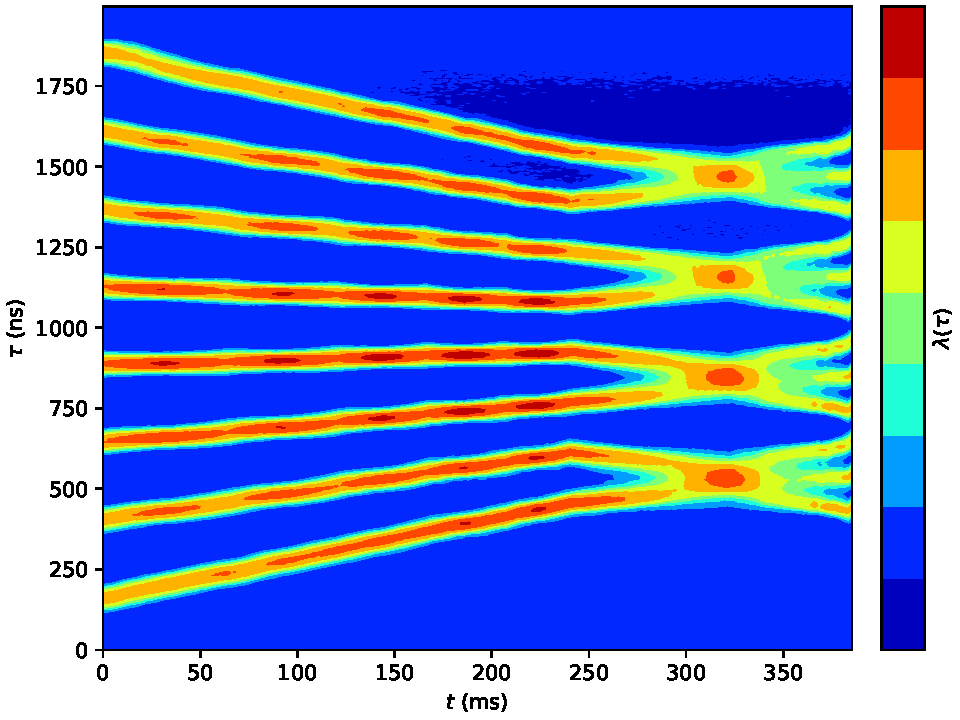
\includegraphics{figs/allmanip.dat.pdf}
    \caption{RF Manipulations conducted in the PS to delay bunch merging until beam is relativistic where space-charge becomes negligible.}
    \label{fig:bcms}
\end{figure}

These manipulations are accomplished by a complicated and dynamic RF ramp scheme as depicted in Figure~\ref{fig:ps_ramp}. This is accomplished through the use of various RF cavities space throughout the PS ring.

\begin{figure}
    \centering
    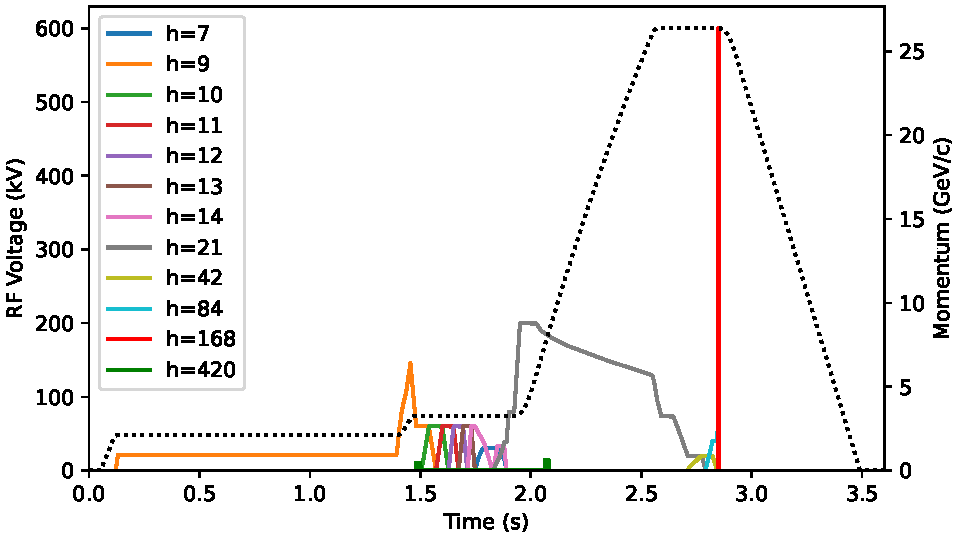
\includegraphics{figs/ps_profiles.pdf}
    \caption{RF harmonic ramp profiles for PS}
    \label{fig:ps_ramp}
\end{figure}

\section{Validation of Longitudinal Space-Charge Trackers}

When current space-charge approximations are incorporated into longitudinal tracking codes such as \href{https://blond.web.cern.ch/}{BLonD} \cite{noauthor_cern_nodate}, we can observe that the bunch length oscillation amplitude and frequency can only be matched when current space-charge calculations are reduced by roughly 30\%, as seen in Figure~\ref{fig:BlonD_v_experiment}. This discrepancy suggests that there may exist an additional stabilizing phenomena within which the current model for longitudinal space-charge impedance is neglecting.

\begin{figure}
    \centering
    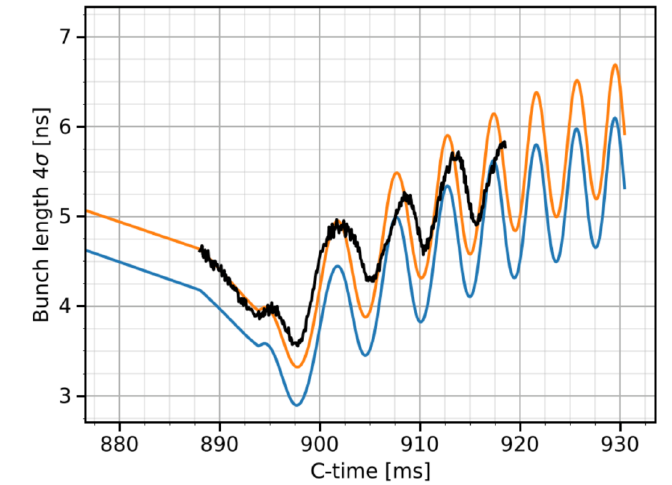
\includegraphics{figs/simulation_v_experiment.png}
    \caption{Bunch length oscillation simulation (orange) benchmarked with experiment (black) \cite{lasheen_longitudinal_2021}.}
    \label{fig:BlonD_v_experiment}
\end{figure}

A possible candidate to describe this discrepancy may be related to the fact that current longitudinal codes neglect transverse betatron motion, suggesting that the variance in individual transverse particle trajectories may lead to describing new phenomena in the longitudinal plane.

\chapter{Beam Dynamics}

This chapter will briefly overview betatron motion in the transverse plane followed by synchrotron motion in the longitudinal plane. Furthermore, bunch wakefields and longitudinal space-charge impedance will be presented to provide context for how particle bunches can destabilize in longitudinal phase-space. The synchrotron frequency, a parameter partially observable by experiment, will be described as will the various ways in which space-charge can affect this quantity.

\section{Transverse Beam Dynamics}

\subsection{Betatron Motion}

A particle's transverse position $u(s)$ (referring to horizontal or vertical transverse positions $x$ and $y$), and derivative $u'(s)=du/ds$, equivalent to particle divergence within a focusing lattice, is characterized by the beta function $\beta(s)$, particle emittance $\epsilon$, and betatron phase $\phi$ so that 
\begin{equation}
    u_\beta(s)=\sqrt{\beta(s)\epsilon}\cos\phi \qquad u_\beta'(s)=-\sqrt{\frac{\epsilon}{\beta(s)}}\left(\alpha(s)\cos\phi+\sin\phi\right)
    \label{eq:hills_equations},
\end{equation} solutions to \textit{Hill's Equations}. The phase advance $\mu(s)$ from a particle's initial phase offset $\mu_0$ is given by
$$\phi = \mu(s) + \mu_0 \qquad \mu(s) = \int_0^s\frac{ds}{\beta(s)}.$$

Accordingly, betatron motion follows elliptical trajectories in ($u$-$u'$) phase-space per it's Twiss parameters $\alpha$, $\beta$ and $\gamma$ \cite{courant_theory_1958} such that $$\epsilon = \gamma u^2 + 2 \alpha u u' + \beta u'^2.$$

Given a continuous beta function $\beta(s)$, the Twiss parameters can be derived: $$\alpha(s) = -\frac{1}{2}\beta'(s) \qquad \gamma(s) = \frac{1+\alpha(s)^2}{\beta(s)}.$$

A particle's relative momentum offset ($dp/p$) or dispersion ($\delta$) can be incorporated with betatron motion by using the dispersion function $D(s)$: $$u(s) = u_\beta + u_D= \sqrt{\beta(s)\epsilon}\cos\phi + D(s)\delta$$ resulting in the total transverse trajectories.

A bivariate transverse distribution ($x$-$x'$, $y$-$y'$) can be statistically described by its covariance matrix $\Sigma$, the product of its ``root-mean-square" emittance $\epsilon$, and the Twiss matrix $\Omega$, encapsulating the focusing properties of the present optics. The statistical emittance $\epsilon$ can be described by the preserved quantity the normalized emittance such that $\epsilon_n=\gamma\beta\epsilon$.

$$\Sigma = \begin{bmatrix}<x^2> & <xx'> \\ <x'x>& <x'^2>\end{bmatrix} = \epsilon\Omega \qquad \Omega = \begin{bmatrix}\beta &-\alpha \\ -\alpha & \gamma\end{bmatrix} \qquad \epsilon = \sqrt{\det(\Sigma)}$$

Such that an injected particle distribution's covariance matrix matches that of the optics $\Omega$, the collective motion of the bunch will be such that the beam width throughout the ring can be described by :
$$\begin{aligned}
        \sigma^2_x(s) & = \beta_x(s)\epsilon_x+D(s)^2\sigma_\delta^2 \\
        \sigma^2_y(s) & = \beta_y(s)\epsilon_y
    \end{aligned}.$$

As consistent in Figure~\ref{fig:ps_transverse_tracking}, individual particle trajectories are seen in faded paths whereas the bulk group motion is described by the \textit{beam envelope} as defined by the \textit{strong focusing} of the beam optics for a matched distribution.

\begin{figure}
    \centering
    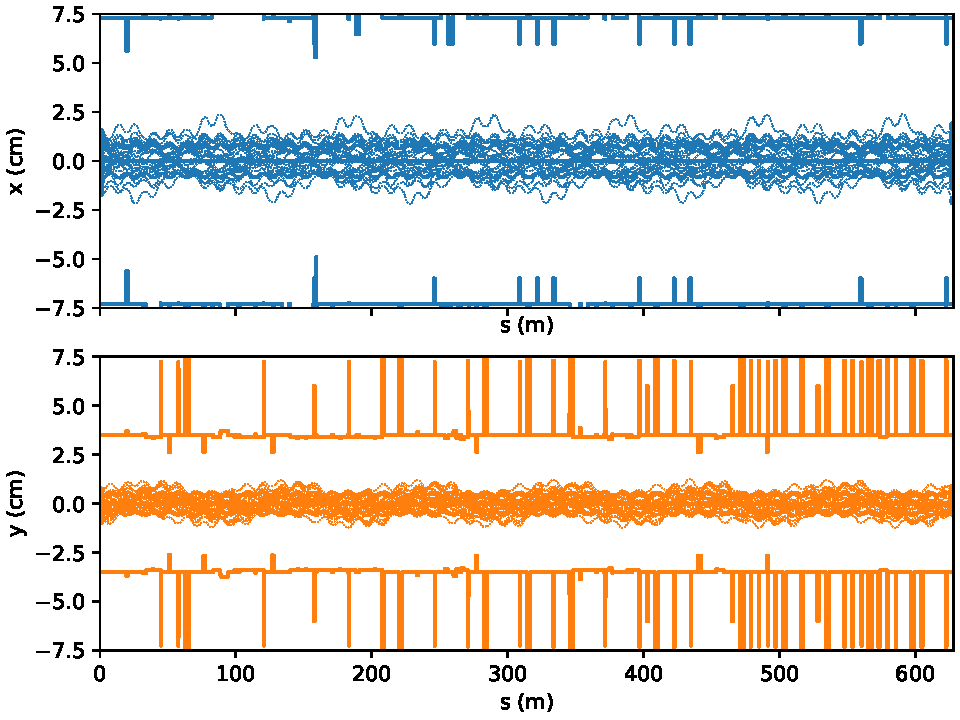
\includegraphics{figs/ps_aperture.multivariate.pdf}
    \caption{Depicted in faded lines, betatron motion is shown for particles propagated through strong focusing optics in the PS. The bulk motion is characterized by the beam envelope in solid lines with respect to the beam pipe aperture.}
    \label{fig:ps_transverse_tracking}
\end{figure}

\section{Longitudinal Beam Dynamics}

\subsection{Single Particle Motion}

As a particle is accelerated in a synchrotron, magnetic dipoles must strengthen to maintain the particle's trajectory as consistent with the magnetic rigidity $$B\rho=\frac{p}{q}$$ where $p$ is particle momentum, $q$ is charge, $\rho$ is bending radius, and $B$ is magnetic dipole field strength. The particle energy gain per turn can be represented by the Panofsky Equation \cite{panofsky_considerations_1956} $$\Delta W = q V_g\sin\varphi$$ where $V_g$ represents the effective RF voltage of a gap, and the RF phase $\varphi$ is defined by $\varphi=h\omega t$ where $h$ is the harmonic number of the RF with respect to the angular velocity $\omega$ of the particle revolution about the ring at absolute time $t$.

If the magnetic field is to be increased at a rate defined by $\dot{B}$, there exists a \textit{synchronous} phase $\varphi_s$ such that the accelerating RF may be modulated so that the bending path of the \textit{synchronous particle} is maintained, given by $$\varphi_s=\arcsin\left(2\pi\rho R\frac{\dot{B}}{V_g}\right)$$ where $R$ defines the characteristic machine radius.

In longitudinal phase-space, it is convenient to work in coordinates relative to the synchronous particle where $$\tau = t - t_s \qquad \delta = \frac{p-p_s}{p_s} \qquad \phi = \varphi - \varphi_s \qquad w = W-W_s$$ define the relative time, momentum, RF phase and kinetic energy of an arbitrary particle with respect to the synchronous particle.

The relative energy \textit{kick} of a particle accelerated through an RF gap is given by
\begin{equation}
    \Delta w = q V(\tau) \qquad
    V(\tau) = V_g g(\phi) \qquad
    g(\phi) = \sin\varphi-\sin\varphi_s.
    \label{eq:kick}
\end{equation}
where the RF gradient $g(\phi)$ yields the following derivative and anti-derivatives $$g'(\phi)=\cos(\varphi_s+\phi) \qquad G(\phi)=(1-\cos\phi)\cos\varphi_s+(\sin\phi-\phi)\sin\varphi_s.$$

In a drift, a particle's revolution period $T$ evolves with total energy $E$ given by \begin{equation}
    \frac{dT}{T} = \frac{\eta}{\beta^2}\frac{dE}{E} \qquad \eta =\alpha- \frac{1}{\gamma^2} \qquad \alpha = \frac{dC/C}{dp/p} = \frac{1}{\gamma_t^2}
    \label{eq:drift}
\end{equation}
where the slippage factor $\eta$ is given by the momentum compaction factor $\alpha$ and the particle's Lorentz factor $\gamma$ defined by it's transition energy $\gamma_t$.

A particle's evolution in phase-space can be described by combining both the kick \eqref{eq:kick} and drift \eqref{eq:drift} equations. For convenience, we introduce the following factor $$\kappa = \frac{\eta}{\beta_s^2E_s}$$ generating the following equations of motion
\begin{equation}
    \dot{\tau} = \kappa w \qquad \dot{w} = \frac{qV(\tau)}{T_s}
    \label{eq:eom}.
\end{equation}

For a linear applied voltage $V(\tau)$ where $V(\tau) \approx V'(\tau)\tau$, the following phase equation for simple harmonic motion can be derived $$\ddot{\tau}+\Omega^2\tau = 0$$ such that the oscillation frequency is given by $$\qquad \Omega^2 = -\frac{\kappa q}{T_s}V'(\tau).$$ Therefore we can identify that the amplitude of our synchrotron oscillation broadly varies with the square of the effective voltage gradient $$\Omega \propto \sqrt{V'(\tau)}.$$

For small-amplitude oscillations where $\phi \to 0$, $g'(\phi) \approx \cos\varphi_s$ therefore $V'(\tau)\approx h\omega_s V_g \cos\varphi_s$ yielding the \textit{Synchrotron Frequency}
\begin{equation}
    \Omega_s^2 = -\frac{h\omega_s^2\eta}{\beta_s^2\gamma_s}\frac{qV_g}{2\pi}\cos\varphi_s
    \label{eq:synchrotron_frequency}.
\end{equation}

\subsection{Hamiltonian Formulation}

Our equations of motion can be derived from the following Hamiltonian
$$\begin{aligned}
        H & = \frac{1}{2}\kappa w^2 -\frac{q}{T_s}\int V(\tau)d\tau \\
          & = \frac{1}{2}\kappa w^2 -\frac{q V_g}{2\pi h}G(\phi)
    \end{aligned}$$ such that Hamilton's equations, $$\frac{dH}{dw} = \dot{\tau} \qquad -\frac{dH}{d\tau} = \dot{w},$$ are obeyed.

A particle's trajectory in phase-space can be represented by $$w(\tau) = \pm \sqrt{\frac{2}{\kappa}\left(H+\frac{q}{T_s}\int V(\tau) d\tau\right)}$$ where the conserved hamiltonion $H$ can be defined by a particles maximum phase-space amplitudes $\hat{\phi}$ and $\hat{w}$ given by
$$H = -\frac{qV_g}{2\pi h}G(\hat{\phi}) = \frac{1}{2}\kappa \hat{w}^2.$$ Given that $\dot{\phi} = h\omega_s\dot{\tau}$ and $W(\phi) = G(\phi)/\cos\varphi_s$, we can define our particle trajectories arbitrarily by $$\dot{\phi} = \Omega_s \sqrt{2(W(\hat{\phi})-W(\phi))}.$$

These trajectories are visualized in Figure~\ref{fig:fisheye}. Particles oscillating near the center with small oscillation amplitudes $\hat{\tau}\to 0$ remain elliptical whereas particles with larger values in $\hat{\tau}$ experience non-linear and asymmetric RF forces, yielding a ``fish" shape.

\begin{figure}
    \centering
    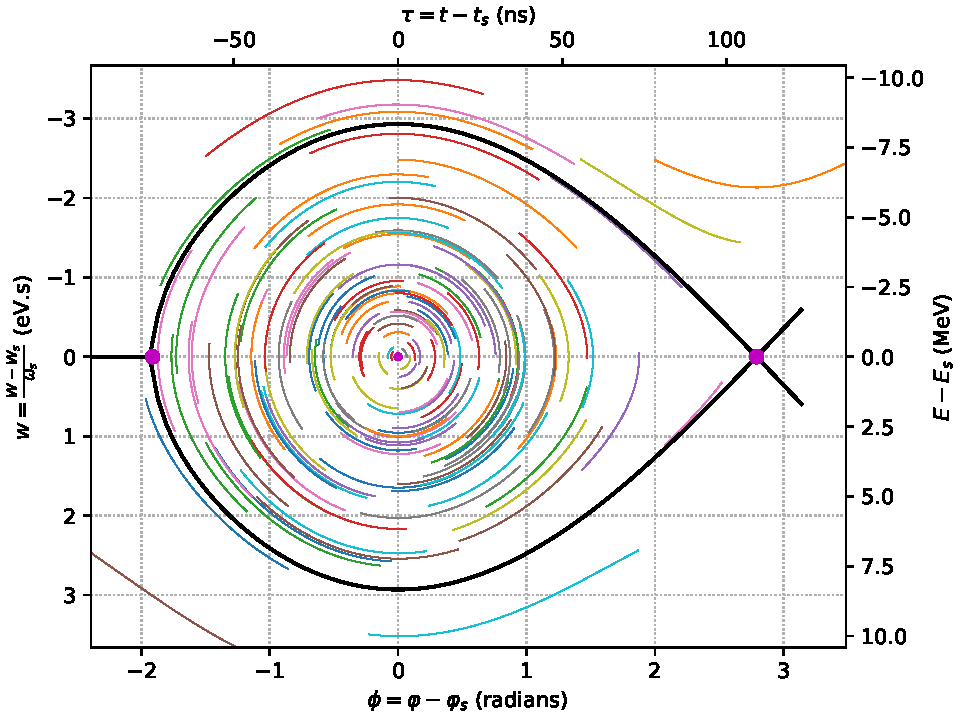
\includegraphics{figs/single_particle_motion/trajectories.pdf}
    \caption{Particles initiated within the separatrix (black contour) circulate along colored elliptical trajectories. Particles initiated outside of the separatrix pursue unbound hyperbolic trajectories.}
    \label{fig:fisheye}
\end{figure}

The separatrix (in black) defines the contour of the Hamiltonian's local maximum such that particles within will retain stable trajectories. Particles present outside the separatrix will follow unstable trajectories.

\subsection{Tune Spread}

The synchrotron period  ($\Pi$) of a particle with given oscillation amplitude $\hat{\phi}$ between the left $\phi_L$ and right $\phi_R$ phase limits is computed by
$$\Pi = \oint \frac{d\phi}{\dot{\phi}} = \frac{2}{\Omega_s}\int_{\phi_L}^{\phi_R} \frac{d\phi}{\sqrt{2(W(\hat{\phi})-W(\phi))}}.$$ 
For a \textit{non-accelerating bucket}, $\varphi_s = 0$, therefore $G(\phi) \to \cos\varphi_s(1-\cos\phi)$, $\phi_R = \hat{\phi}$ and $\phi_L = -\hat{\phi}$ resulting in
$$\Pi = \frac{4}{\Omega_s\sqrt{2}}\int_0^{\hat{\phi}}\frac{d\phi}{\sqrt{\cos\phi-\cos\hat{\phi}}} = \frac{4K(\hat{\phi}/2; k=\csc(\hat{\phi}/2))}{\Omega_s}.$$
If we define the normalized synchrotron tune $\mu$ as $\mu = \Omega(\hat{\phi})/\Omega_s$, by Taylor series expansion we produce
\begin{equation}
    \mu =\frac{\pi}{2K(\frac{\hat{\phi}}{2})} \approx 1-\frac{\hat{\phi}^2}{16} +\mathcal{O}(\hat{\phi}^4) \qquad \phi \approx 4\sqrt{1-\mu}
    \label{eq:tune_spread}.
\end{equation}
Accordingly, a distribution of linear charge density $\lambda(\phi)$ an be associated to a spread in normalized synchrotron tune $\mu$ as displayed in Table~\ref{tab:freq_spread} and depicted in Figure~\ref{fig:tune_spread}.

\begin{table}
    \centering
    \begin{tabular}{c|c|c|c}
                  & $\lambda(\phi)$                                                                                                   & $\lambda(\mu)$                                                                              & $d\lambda/d\phi$                      \\
        \hline
        Gaussian  & $\frac{1}{\sigma_{\hat{\phi}}\sqrt{2\pi}}\exp\left(-\frac{1}{2}\frac{\hat{\phi}^2}{\sigma_{\hat{\phi}}^2}\right)$ & $\frac{1}{\sigma_{\hat{\phi}}\sqrt{2\pi}}\exp(-\frac{1}{2}\frac{16(1-\mu)}{\sigma_\phi^2})$ & $-\frac{\phi}{\sigma^2}\lambda(\phi)$ \\
        Parabolic & $\frac{3}{2L_{\hat{\phi}}}(1-4\frac{\hat{\phi}^2}{L_{\hat{\phi^2}}})$                                             & $\frac{3}{2L^3}(L^2-64+64\mu)$                                                              & $-\frac{12\phi}{L^3}$                 \\
    \end{tabular}
    \caption{Impact of longitudinal distribution on synchrotron frequency spread.}
    \label{tab:freq_spread}
\end{table}

\begin{figure}
    \centering
    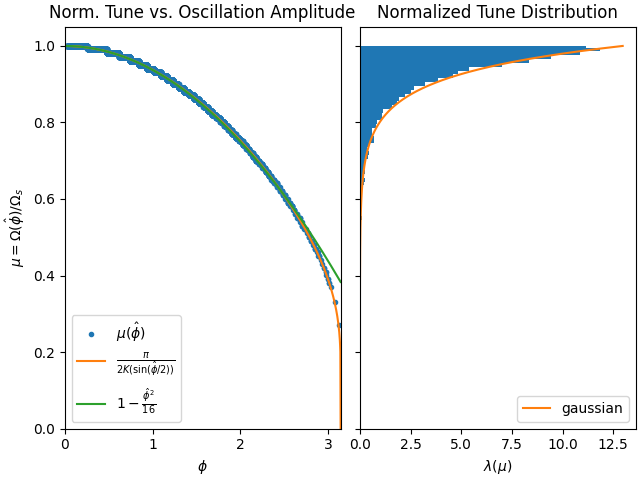
\includegraphics{figs/single_particle_motion/normalized_tune.png}
    \caption{Spread of synchrotron tune with oscillation amplitude}
    \label{fig:tune_spread}
\end{figure}

\section{Longitudinal Space Charge}

The previous section describes the synchrotron motion of independent particles to circulate within a quasi-elliptical RF bucket. The electromagnetic interaction between particles was neglected and accordingly will be accounted for in the following section. Firstly, the interaction between a particle's electromagnetic fields and the surrounding conductive aperture, ie: the beam pipe, will be formalized as a wakefield effect of reactive impedance sources. Additionally the self-interaction of charged particles within a bunch can be described as a space-charge impedance and represented as a similar wakefield phenomenon.

\subsection{Wakefields}

Consider charged particles in a bunch passing through a discontinuity in a conductive aperture. The discontinuity will perturb the emitted electromagnetic fields trailing the bunch and form wakefields that will induce a voltage on the following particles. This induced voltage can be given by the convolution of the linear charge density $\lambda(\tau)$ and the wake function $\mathcal{W}(\tau)$ given by \cite{wiedemann_particle_2015,zotter_impedances_1998}
$$\Delta V(\tau)=-\int_0^\infty\lambda(t)\mathcal{W}(\tau-t)dt=-\mathcal{W}*\lambda$$
where the bunch's longitudinal charge profile $\lambda(\tau)$ is normalized to the total charge $Q=qN_b$ such that $$Q = \int_{-\infty}^\infty \lambda(\tau) d\tau.$$

We can define the impedance $Z(f)$ and spectrum $S(f)$ from the Fourier transforms of the wake function $\mathcal{W}(\tau)$ and charge profile $\lambda(\tau)$ respectively given by
$$Z(f)  =\int_{-\infty}^\infty\mathcal{W}(\tau)e^{-i\omega\tau}d\tau \qquad S(f)  =\int_{-\infty}^\infty\lambda(\tau)e^{-i\omega\tau}d\tau.$$
The convolution of the wake function and linear charge density can be written as the inverse Fourier transform of the product of the spectrum and the impedance, therefore the induced voltage can be re-written as
$$\Delta V(\tau)=-\int_{-\infty}^\infty S(f)Z(f)e^{i\omega \tau}df.$$

For a linear reactive impedance source such that $Z/n$ is constant, where $n = f/f_s$, the impedance term can be separated from the integral so that the inverse Fourier transform of the spectrum can be incorporated instead as the derivative of the linear charge density
\begin{equation}
    \Delta V=\frac{-i}{\omega_s}\frac{Z}{n}\frac{d\lambda}{d\tau}
    \label{eq:induced_voltage}.
\end{equation}

\subsection{Space Charge Impedance}

The relativistic longitudinal self fields of a particle of a long narrow beam can be defined by \cite{ferrario_space_2014}
$$E_z=-\frac{\bar{g}}{2\pi\epsilon_0\gamma^2}\frac{\partial \lambda}{\partial z},$$
where the \textit{geometry factor} $\bar{g}$ is defined by (\ref{eq:longitudinal_self_fields})
$$\bar{g}=\int_r^b\frac{f(r')}{r'}dr'\qquad f(r)=\frac{\int_0^r\rho(r')r'dr'}{\int_0^\infty\rho(r')r'dr'}=\frac{Q'}{Q}.$$
Here Q' defines the amount of charge enclosed within the radius $r$. Averaged about a particle's revolution during one turn, these self fields will induce a voltage that can be defined as the \textit{Longitudinal Space-Charge Impedance}  given by \cite{lee_accelerator_2004}
\begin{equation}
    \frac{Z}{n} = -i\frac{Z_0}{\beta\gamma^2}\bar{g}
    \label{eq:space_charge_impedance}.
\end{equation}

The space-charge impedance can therefore be used to characterize the effective voltage drop of particles within a bunch by combining Equations \ref{eq:induced_voltage} and  \ref{eq:space_charge_impedance} to yield our induced space-charge voltage $\Delta V_{SC}$ as a function of the derivative of linear charge density profile and the geometry factor.

\begin{equation}
    \Delta V_{SC} = -\frac{d\lambda}{d\tau}\frac{Z_0}{\beta_s\gamma_s^2}\frac{\bar{g}}{\omega_s}
    \label{eq:v_sc}
\end{equation}

The geometry factors as a function of transverse radial position $\bar{g}(r)$ for a uniform (\ref{eq:g_uniform}), parabolic (\ref{eq:g_parabolic}) and gaussian (\ref{eq:g_gaussian}) are depicted in Figure~\ref{fig:geometry_factors}.
\begin{figure}
    \centering
    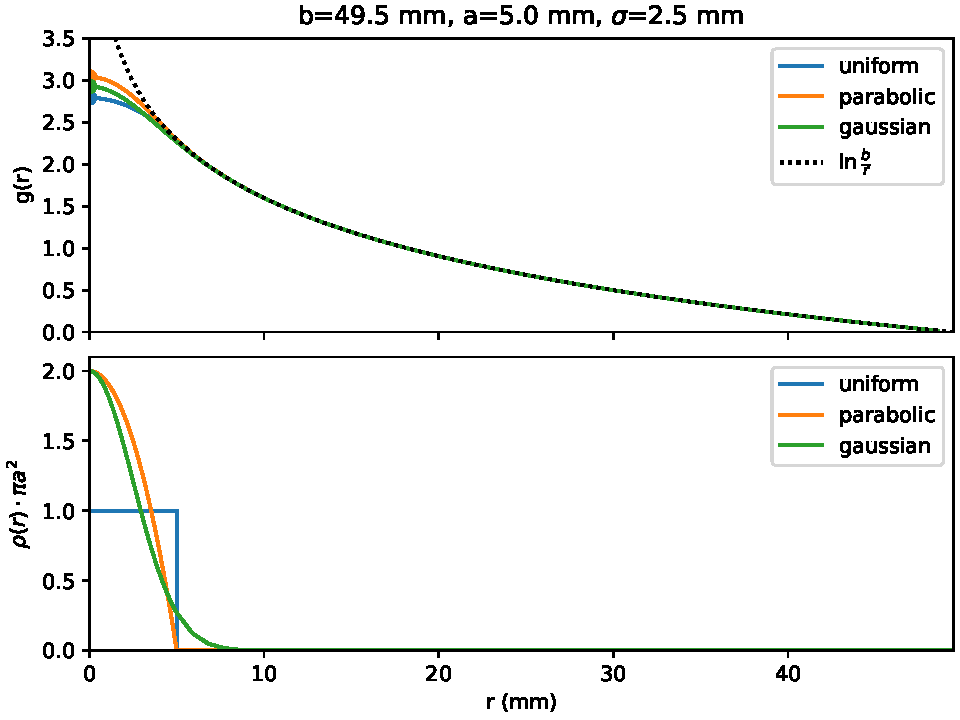
\includegraphics{./figs/geometric_factors.pdf}
    \caption{Geometric factors for uniform, parabolic and gaussian charge profiles, sized with equivalent variances ($\sigma = a/2 = L/4$), with aperture radius $b$.}
    \label{fig:geometry_factors}
\end{figure}
We observe that the shape of geometry factors for uniform, parabolic or gaussian beams with similar variances is mostly preserved. The geometry factor describing a uniform circular bunch of radius $a$ in conducting aperture of radius $b$ is given by $$\bar{g}(r)=\frac{1}{2}+\ln\frac{b}{a}-\frac{1}{2}\frac{r^2}{a^2}.$$
The maximum geometry factor, $\bar{g}(r=0)$, corresponds to maximum longitudinal space-charge effects. Particles with large dispersion ($\delta$) or transverse emittance ($\epsilon_\perp$) will follow misaligned betatron trajectories with non-zero effective radial position, and therefore will incur reduced space-charge effects as consistent with \eqref{eq:v_sc}.

\subsection{Tune Shift}

Relevant to the oscillation frequency, it is also worth defining the space-charge impedance voltage gradient \begin{equation}
    V'_{SC}(\tau) = \frac{Z_0}{\beta_s\gamma_s^2}\frac{\bar{g}}{\omega_s}\frac{d^2\lambda}{d\tau^2}.
\end{equation} The \textit{normalized tune shift} due to space-charge impedance is therefore
\begin{equation}
    \mu = \frac{\Omega}{\Omega_s} = \sqrt{1 + \frac{V'_{SC}}{V'_{RF}} }= \sqrt{1 +\zeta\Lambda}
    \label{eq:tune_shift},
\end{equation} 
where $\zeta$ is given by the maximum space-charge impedance and $\Lambda$ describes variation in geometry factor on account of transverse motion
$$\zeta = \frac{V'_{SC}(r=0)}{V'_{RF}} \qquad \Lambda = \frac{\bar{g}}{\bar{g}(r=0)}.$$

Considering a parabolic charge distribution where
$$\lambda(\tau)=\frac{3Q}{2L_\tau}\left(1-4\frac{\tau^2}{L_\tau^2}\right) \qquad |\tau| < \frac{L_\tau}{2},$$
the charge gradient is therefore given by $$\frac{d\lambda}{d\tau} = \frac{-12Q}{L_\tau^3}\tau$$ The induced voltage gradient of a parabolic bunch due to space charge is given by  \cite{lasheen_longitudinal_2016} \begin{equation}
    V'_{SC} = -\frac{12Q}{\omega_s}\frac{\Im (Z)}{n}\frac{1}{L_\tau^3}=-\frac{12Q}{\omega_s}\frac{Z_0}{\beta_s\gamma_s^2}\frac{\bar{g}}{L_\tau^3}
    \label{eq:vp_sc}.
\end{equation} 
We see that $\zeta$ is therefore a constant throughout longitudinal phase-space, modulated only by the RF gradient $V'_{RF}(\tau)$. For the on-axis particle where $\Lambda=1$, the synchrotron frequency will experience a uniform shift due to space-charge as observed in the tune distributions seen in Figure~\ref{fig:tune_shift}. Here we have assumed a uniform space-charge geometry factor neglecting betatron motion and varying aperture size, both to be addressed in the following chapters.

\begin{figure}
    \centering
    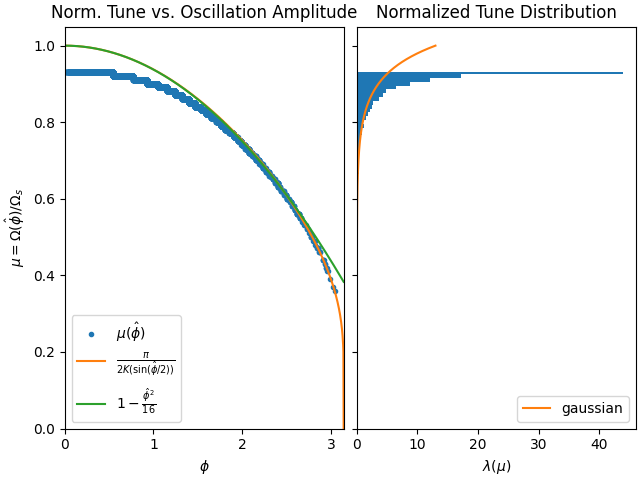
\includegraphics{figs/tune_shift/normalized_tune.png}
    \caption{Space-charge tune shift for 30 ns bunch, 2.08e12 protons, bunch}
    \label{fig:tune_shift}
\end{figure}

\chapter{Aperture Reconstruction}

\section{Introduction}

As discussed in the previous chapter, the effects of longitudinal space-charge impedance is described in part by a characteristic geometry factor, describing the induced longitudinal fields due to the position a particle occupies within a transverse bunch distribution in a finite conducting aperture. To re-iterate, the geometry factor describing the longitudinal fields felt of a particle within a uniform cylindrical bunch can be described by
$$\bar{g}(r) = \frac{1}{2} + \ln\frac{b}{a}-\frac{1}{2}\frac{r^2}{a^2}.$$

Much of this work revolves on accurately tracking and characterizing the beam size ($a$) and particle radius ($r$) relevant to this equation, however the PS's model for beam pipe aperture ($b$) is of unknown precision and many years out of date, (circa 2013) to wit the updating of said aperture profile by manual tallying is time consuming, tedious, and error prone.
\begin{figure}
    \centering
    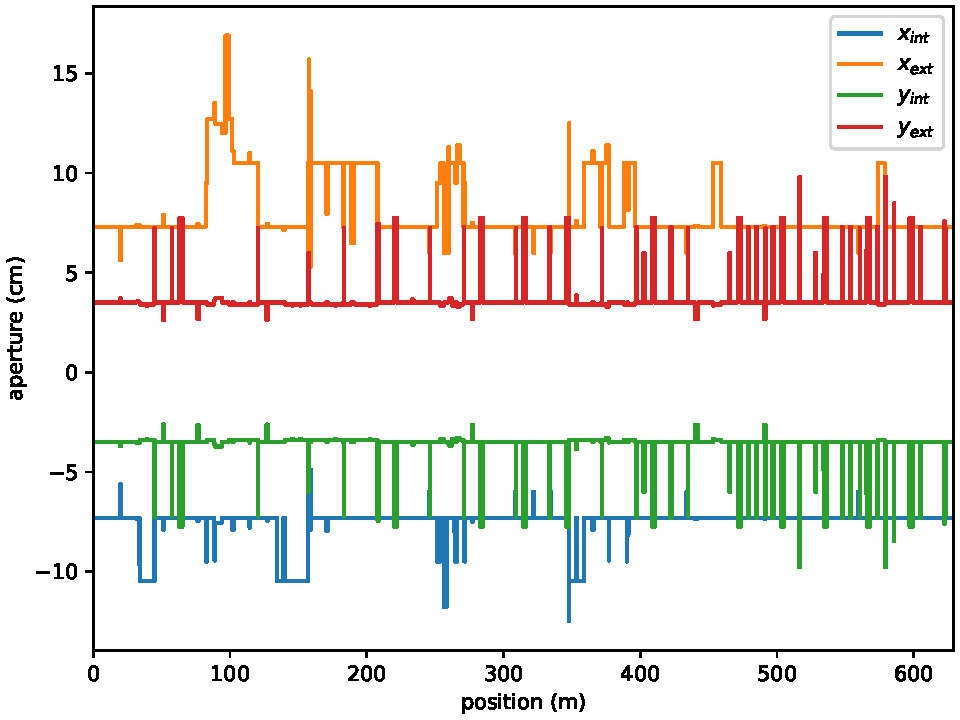
\includegraphics{figs/ps_aperture.pdf}
    \caption{Current aperture model of PS, last updated in 2013}
    \label{fig:ps_aperture_model}
\end{figure}
The most recent model, as depicted in Figure~\ref{fig:ps_aperture_model}, is old and assumes for elliptical geometries. Though this is mostly valid for most of the ring, being an elliptical beam pipe, 35 x 73 mm wide, there are numerous nuanced cross sections of varying components such as septa, bellows, pump-out ports, etc. whose electrical boundaries aren't incorporated into this model.

\section{Linearizing a Synchrotron}

The PS and it's sub-assemblies can be conveniently represented as triangular meshes, portable in STL (stereo-lithography) files, as depicted in Figure~\ref{fig:ps_mu}.
\begin{figure}
    \centering
    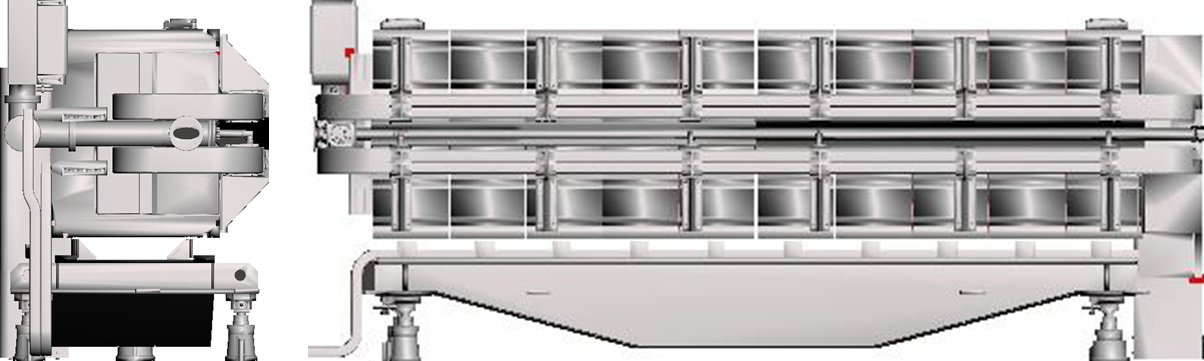
\includegraphics{figs/ps_magnet.png}
    \caption{Triangular mesh representation (front and right views) of a PS Dipole Magnet Unit (MU)}
    \label{fig:ps_mu}
\end{figure}

The first objective is to define a reference-trajectory $R(\phi)$ in curvilinear coordinates consistent with a ``Frenet-Serret" coordinate system  such that a torus can be ``inflated" until collision with the electrical aperture of the model are identified. Our cartesian model can be described by toroidal coordinates ($r,\theta,\phi$) from:
$$\begin{aligned}
        x & = (R(\phi)+r\cos\theta)\cos\phi \\
        y & = (R(\phi)+r\cos\theta)\sin\phi \\
        z & = r\sin\theta,
    \end{aligned}$$
where $R(\phi)$ serves the reference radius as is defined by the geometry of the PS's 100 straight sections (SS) and 100 magnet units (MU). A schematic of the reference trajectory for one of the PS's 36$^\circ$ sub-sectors is depicted belpw in Figure~\ref{fig:ref_traj}.
\begin{figure}
    \centering
    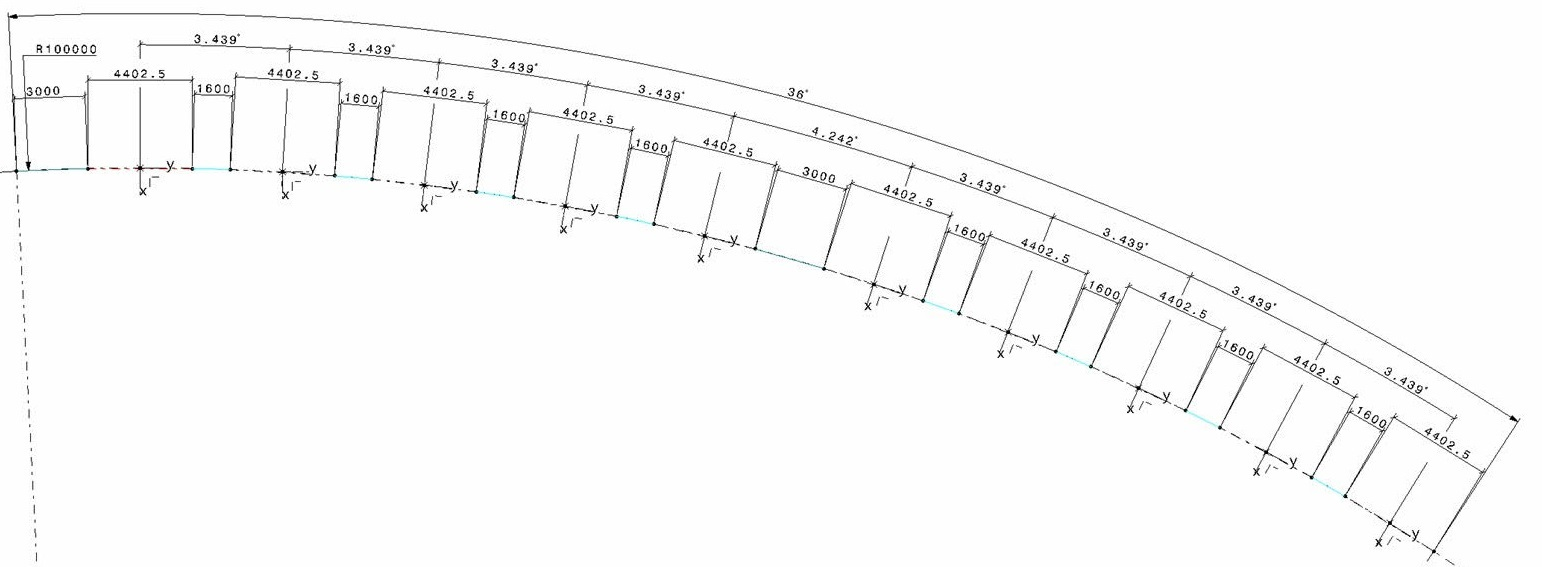
\includegraphics{figs/reference_trajectory_path.jpg}
    \caption{Engineering drawing of reference trajectory in a PS sector}
    \label{fig:ref_traj}
\end{figure}

We can use this definition of reference trajectory $R(\phi)$ to ``unwrap" the PS ring model into equivalent \textit{linearized}, transforming our model coordinates into curvilinear $(x, y, s)$ and so to detect the aperture, a straight cylinder originating about the reference trajectory needs to be "inflated" until an intersection between surfaces is detected and recorded.
\begin{figure}
    \centering
    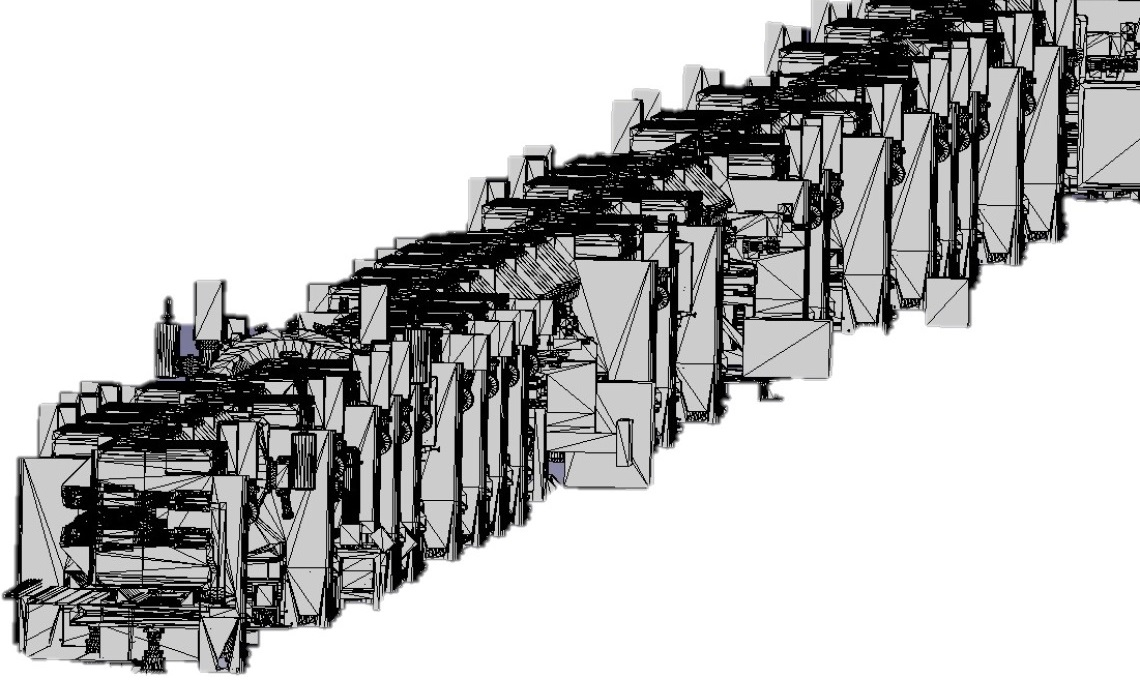
\includegraphics{figs/ps_linac.png}
    \label{fig:ps_linac}
    \caption{Example of the PS model in \textit{linearized} form, transformed to curvilinear coordinates (x, y, s).}
\end{figure}

\section{Ray Casting}

To perform this virtual \textit{inflation} of our collision surface with the mechanical model, the \textit{Möller–Trumbore} intersection algorithm can be used to compute intersection angles with the PS \cite{moller_fast_1997}. It is commonly used in 3D graphics to efficiently detect and compute the intersection between light rays and polygons as well is it easily parallelized. In Figure  \ref{fig:ray_casting}, a point source is cast through a spherical shell to demonstrate the technique. The algorithm is able to evaluate each light ray with all faces to determine if an intersection is possible and if so, where. Details for this algorithm are elucidated in Appendix \ref{eq:moller}.

\begin{figure}
    \centering
    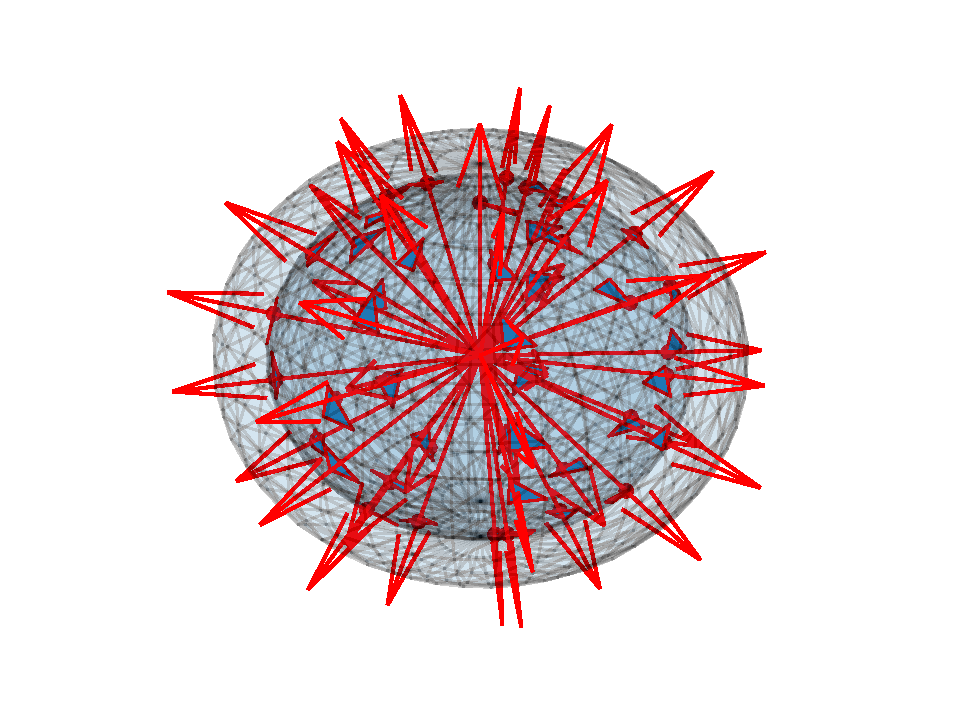
\includegraphics{figs/shell.pdf}
    \caption{Rays originating from a point source are cast through a spherical shell. Intersecting faces are outlined in red with intersection point indicated by red markers.}
    \label{fig:ray_casting}
\end{figure}

\section{Reconstruction Quality}

After transforming the cartesian mechanical model of the PS to curvilinear coordinates, a line source was ``illuminated" along the central beam path whose ray intersections were detected. These illuminations were performed on each of the 100 magnet units and straight sections individually and then combined to produced an updated and detailed aperture as depicted in \ref{fig:ps_aperture}. The distinctive colors of the newly defined aperture coincide with a preservation for component granularity, being able to attribute specific aperture coordinates along the beam path with a particular magnet unit or straight section, allowing for easy verification.

\begin{figure}
    \centering
    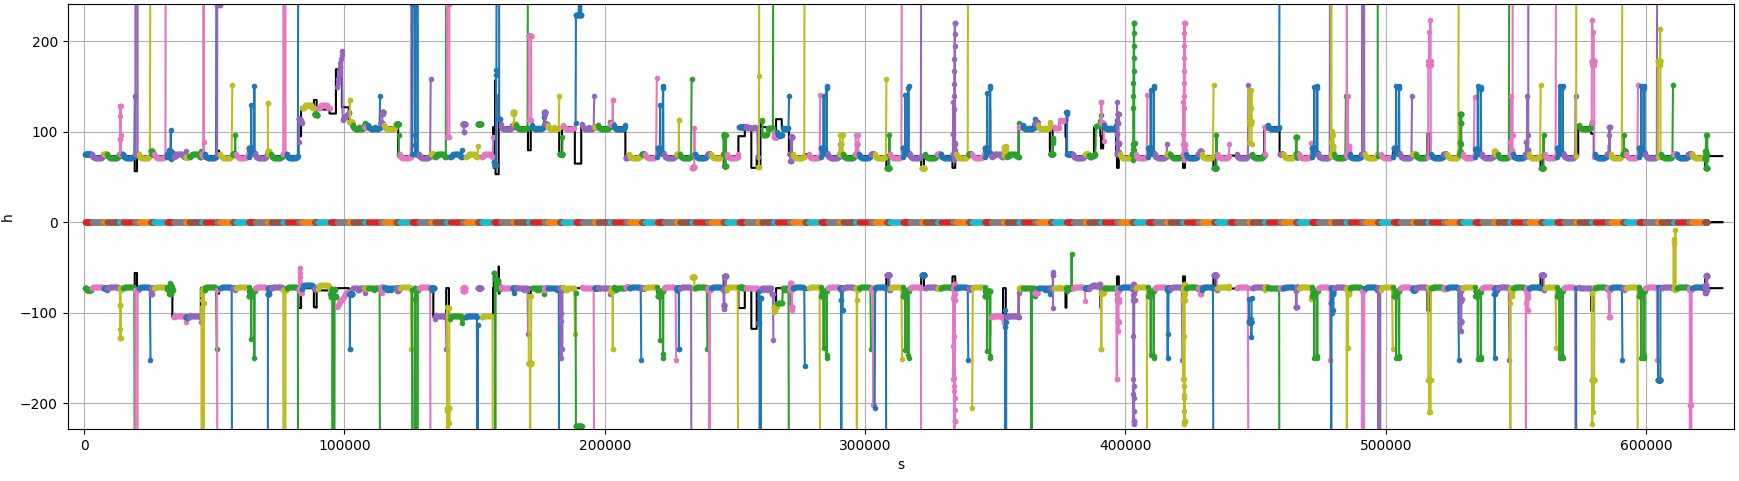
\includegraphics[width=\linewidth]{figs/ps_aperture.png}
    \caption{Horizontal aperture of the reconstructed PS aperture by Ray-Casting, superimposed atop the 2013 model (black)}
    \label{fig:ps_aperture}
\end{figure}

By using this automated technique as opposed to manually generating an aperture, details could be queried at much higher longitudinal and poloidal resolutions, as seen in Figure~\ref{fig:ps_aperture_hi_res}. Additionally, features for smaller and yet frequent discrepancies could be automatically identified as in the case of pump-out ports and bellows.

\begin{figure}
    \centering
    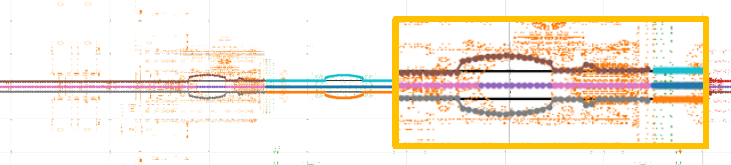
\includegraphics{figs/apertture_hi_res.PNG}
    \caption{Hi-Res reconstruction of PS aperture}
    \label{fig:ps_aperture_hi_res}
\end{figure}

Additionally, details of RF cavities, diagnostic ports and septa can be compared with that of the older model per Figure~\ref{fig:ps_septa}.

\begin{figure}
    \centering
    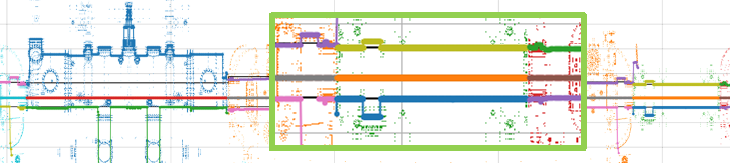
\includegraphics{figs/aperture_comparison.PNG}
    \caption{Comparison of updated aperture model with 2013 version (black)}
    \label{fig:ps_septa}
\end{figure}

In summary, it has been shown that a high resolution aperture of the PS can be automatically generated to be consistent with the 3D CAD model generated by the mechanical team. This model can be conveniently imported when changes are made, or on an automatic basis. This aperture will contain much more detail than likely necessary for the purposed of longitudinal-space charge studies, however this procedure may allow for the approximation of no-elliptical geometries.

\chapter{Simulation}

\section{Transverse Tracking}

The optics of the PS are described by the beta function ($\beta(s)$ and dispersion function $D(s)$ as depicted in Figure~\ref{fig:ps_optics}.

\begin{figure}
    \centering
    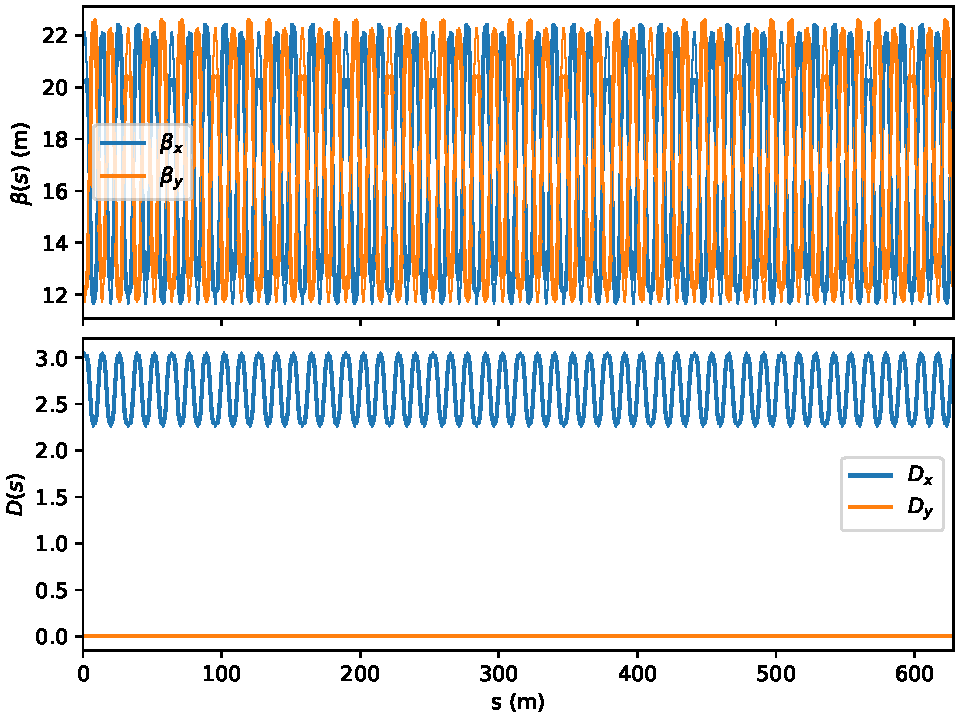
\includegraphics{figs/ps_optics.pdf}
    \caption{Transverse optics of the PS}
    \label{fig:ps_optics}
\end{figure}

For simplicity of transverse tracking purposes and subsequent development of analytic relationships, the periodicity of these optics can be accurately represented as a two-term Fourier series
\begin{equation}
    \beta(\theta) \approx \sum_k \beta_k e^{i k\theta} \qquad D(\theta) \approx \sum_k D_k e^{i k\theta}
    \label{eq:optics_decomposition}
\end{equation}
whose coefficients are described in Table~\ref{tab:ps_optics_fourier}. This approximation reduced the computation time for the subsequent transverse tracking simulations and helped avoid interpolation artifacts.

\begin{table}
    \centering
    \begin{tabular}{c | c  r | c  r }
        $\beta_x(\theta)$ & $\beta_{0,x}$ & 16.89 & $\beta_{50,x}$ & +4.43-2.84i \\
        $\beta_y(\theta)$ & $\beta_{0,y}$ & 17.01 & $\beta_{50,y}$ & -4.46+2.86i \\
        $D_x(\theta)$     & $D_{0,x}$     & 2.66  & $D_{50,x}$     & +0.34-0.22i \\
        $D_y(\theta)$     & $D_{0,y}$     & 0     & $D_{50,y}$     & 0           \\
    \end{tabular}
    \caption{Primary Fourier coefficients describing periodic nature of PS optics}
    \label{tab:ps_optics_fourier}
\end{table}

A transverse tracker was developed to solve for betatron trajectories described by solutions to Hill's Equations (Equations  \ref{eq:hills_equations}). A bivariate gaussian distribution with matching covariance matrix ($\Sigma$) to that of the PS's Twiss matrix ($\Omega$) was ``injected" and tracked about one turn in the synchrotron as depicted in Figure~\ref{fig:trans_tracking}.

\begin{figure}
    \centering
    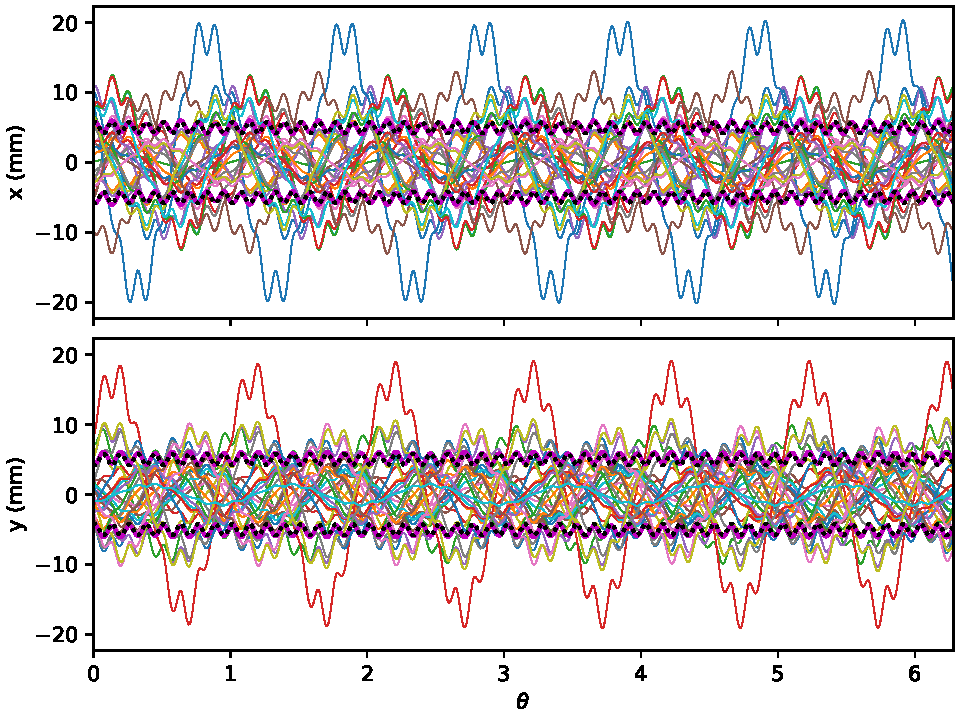
\includegraphics{figs/tracking.pdf}
    \caption{Faded trajectories of select particles alongside statistical (magenta) and analytic (black) beam widths in the PS.}
    \label{fig:trans_tracking}
\end{figure}

\subsection{Effective Geometry Factor}

Given the ability to track the transverse locations of individual particles propagating through the PS lattice relative to the transverse particle distribution itself, each particle's geometry factor can be computed and observed to vary along the ring. These geometry factors can be averaged resulting in the definition of the effective geometry factor, characterizing the particle's turn-averaged experienced space-charge, dependent on the optics, aperture, and the particle's characteristic emittance, phase advance and dispersion.

$$\bar{g}_{eff} \propto \bar{g}(\epsilon_\perp, \mu_0, \delta)$$

The transverse tracker was accordingly used to build a response matrix to predict a particle's effective geometry factor given it's initial conditions ($\epsilon_x, \epsilon_y, \delta$) within a known beam of characteristic statistical emittance and width ($\epsilon_\perp, \sigma_\delta$). In relation to dispersion, Figure~\ref{fig:g_eff_dispersion} indicates a parabolic dependence with the effective geometry factor and a linear relationship with transverse emittance. A particle's phase-advance appears to have minimal impact on the effective geometry factor.

$$\bar{g}_{eff} \propto \bar{g}_{max} - C_0\delta^2 - C_1\epsilon_x - C_2\epsilon_y$$

\begin{figure}
    \centering
    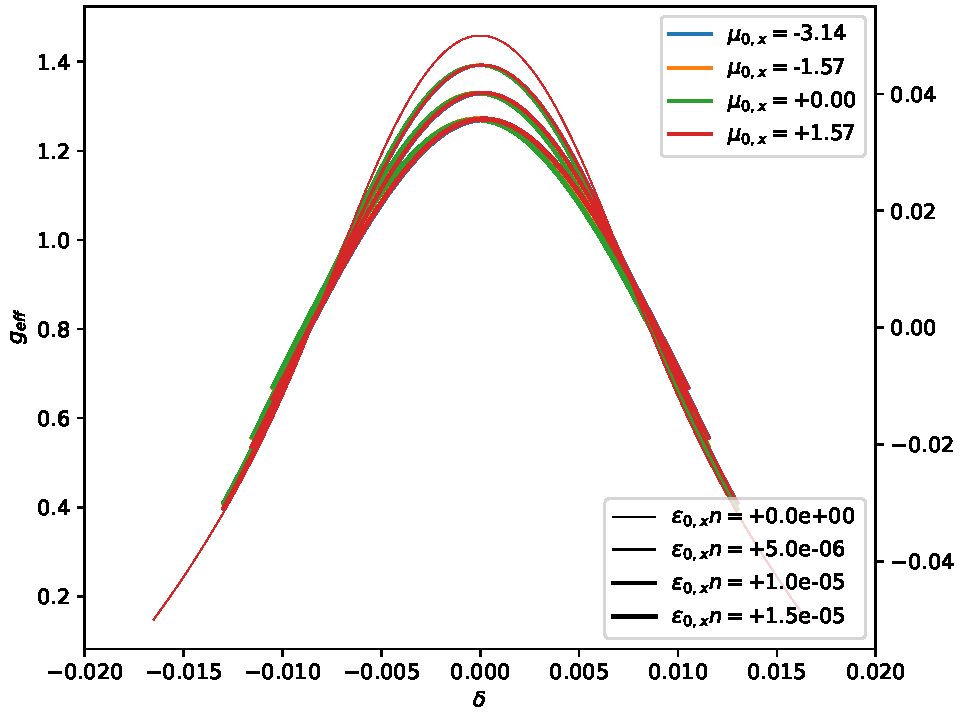
\includegraphics{figs/g_dispersion.pdf}
    \caption{Impact of particle \textbf{dispersion} on effective geometry factor}
    \label{fig:g_eff_dispersion}
\end{figure}

We see however that the domain for $\bar{g}_{eff}$ is limited as particles with a combination of very high dispersion or very high emittance are will collide with the beam aperture and be lost. This phenomena is more readily visible in Figure~\ref{fig:g_emittance} where we see the thicker lines (representing higher dispersion) end up being truncated with increased transverse emittance. This figure also more clearly elucidates the exponential relationship between emittance and the geometric factor when dispersion is low.

\begin{figure}
    \centering
    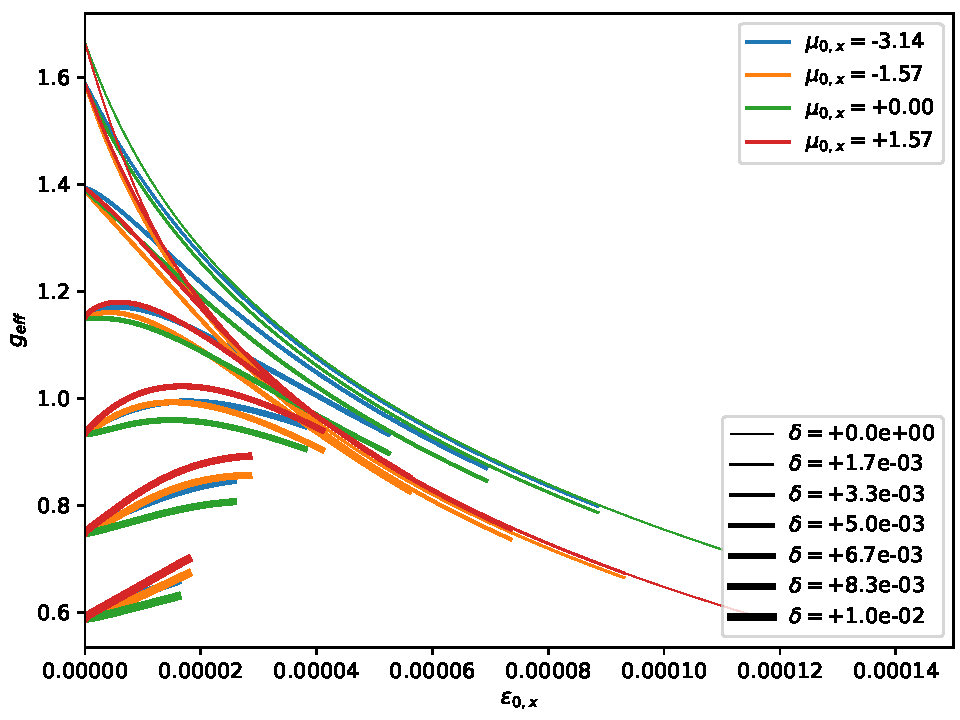
\includegraphics{figs/g_emittance.pdf}
    \caption{Impact of particle \textbf{emittance} on effective geometry factor}
    \label{fig:g_emittance}
\end{figure}

We see in Figure~\ref{fig:g_phase_advance} that though changes in geometry factor are dominated by dispersion and particle emittance, along the course of a particle around it's elliptical trajectory in transverse phase-space, there will be a sinusoidal impact on the geometry factor due to betatron phase-advance, though this can largely be neglected.

\begin{figure}
    \centering
    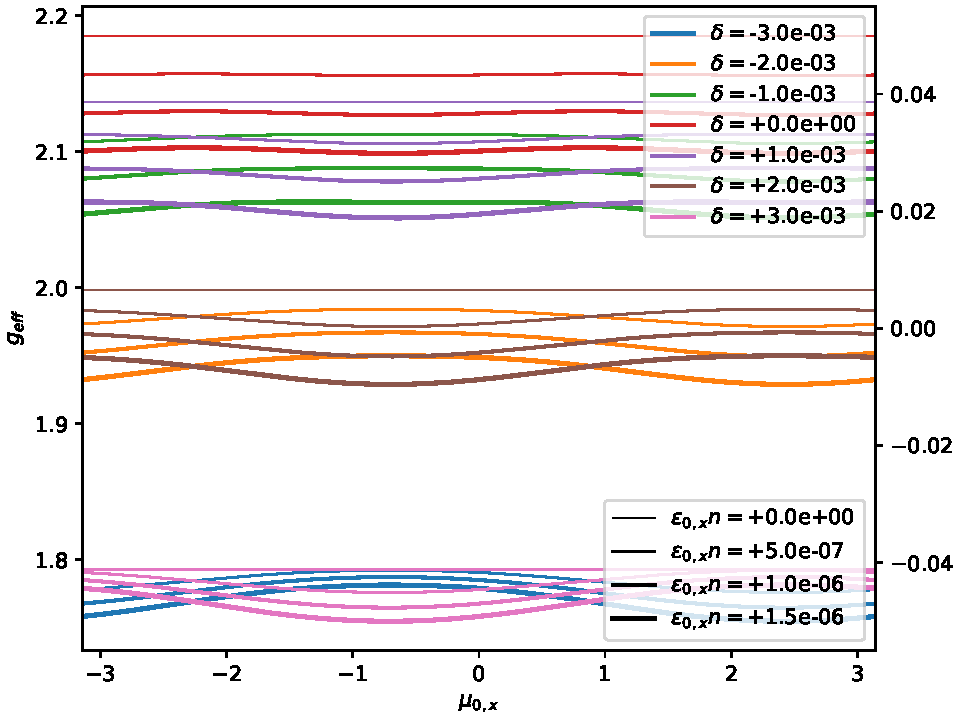
\includegraphics{figs/g_phase_advance.pdf}
    \caption{Impact of particle \textbf{phase advance} on effective geometry factor}
    \label{fig:g_phase_advance}
\end{figure}

These relationships can be summarized in a lookup table represented as a response matrix, visualized in Figure~\ref{fig:g_eff_vol}.

\begin{figure}
    \centering
    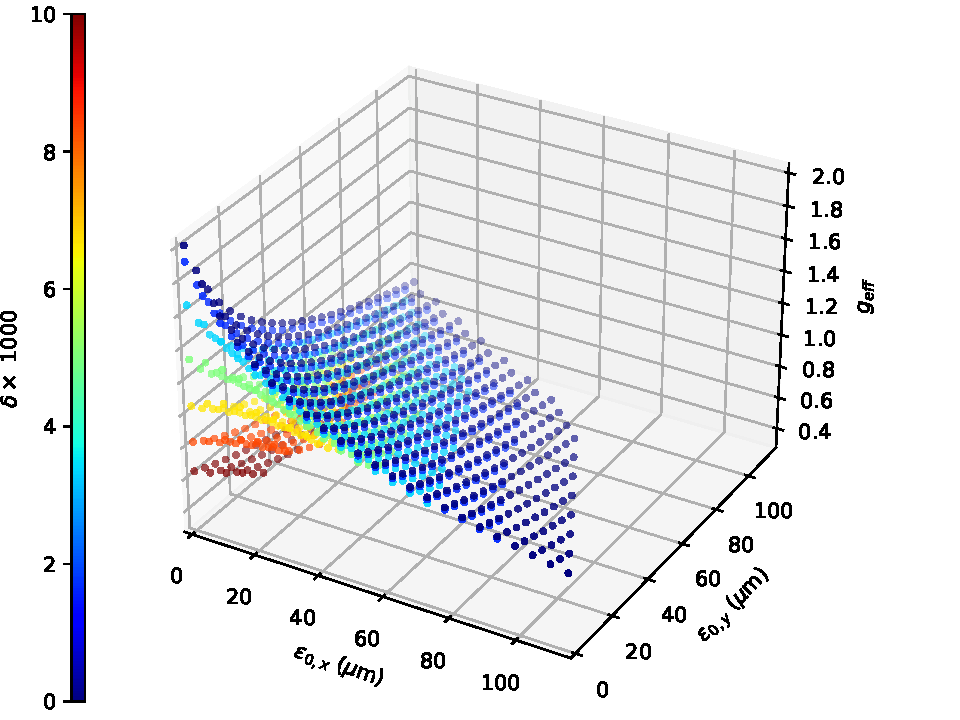
\includegraphics{figs/g_eff.surface.0.pdf}
    \caption{Multi-dimensional vector space of effective geometry factor for a particle of known transverse emittance and dispersion.}
    \label{fig:g_eff_vol}
\end{figure}

The impact of particle phase-advance was neglected as it's effect are minimal in comparison to the other dependencies on account of the fact that the transverse tune is large and accordingly a variation in a particle's initial phase-offset will contribute to little variance in the particle's effective radial position.

\section{Longitudinal Tracking}

\subsection{Usage of Geometric Factor}

A longitudinal tracker can be developed by discretizing Equations \ref{eq:eom}, yielding the \textit{turn-by turn} ``kick" and ``drift" components respectively
$$w_{i+1}-w_i \to \Delta w = qV(\tau) \qquad \tau_{i+1}-\tau_i \to \Delta\tau = \kappa T_s w.$$
To include space-charge in our tracker, the induced voltage due to space-charge impedance is include with RF acceleration by
$$V(\tau) = V_{RF} + V_{SC}.$$
The geometric factor $\bar{g}$ is replaced as found in \eqref{eq:space_charge_impedance} with the effective particle dependent geometry factor $\bar{g}_{eff}$ for a parabolic longitudinal bunch given by
$$V_{SC} = -\frac{12Q}{L_\tau^2}\frac{Z_0}{\beta\gamma^3}\frac{g_{eff}(\epsilon_x,\epsilon_y,\delta)}{\omega_s}.$$

Transverse emittance $\epsilon_x$ and $\epsilon_y$ is presumed to be preserved between synchrotron ``kicks", however dispersion evolves with synchrotron motion and accordingly the geometry factor will notice an influence as the particle orbits in longitudinal phase-space.

\subsection{Tune ``Blur"}

Consider we sample our distribution from a 6D ellipsoidal distribution associated with gaussian transverse emittance ($\epsilon_\perp$), uniform betatron phase advance ($\mu_0$), and gaussian dispersion ($\sigma_\delta$) and bunch length ($\sigma_\tau$). Using this modified longitudinal tracker, the normalized tune distribution incorporating the effective geometry factor due to transverse motion is given by Figure~\ref{fig:tune_blurr} where we observe a ``blurred'' tune spread distribution for the synchrotron frequency.

\begin{figure}
    \centering
    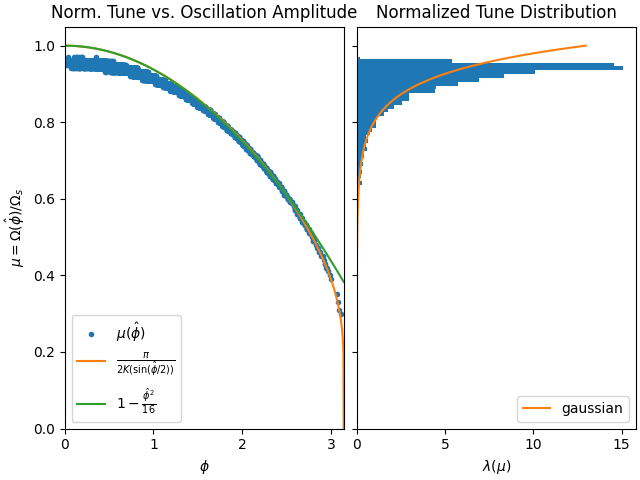
\includegraphics{figs/tune_blurr/blurred_tune.png}
    \caption{Blurred Synchrotron Frequency spread distribution due to space-charge impedance with transverse motion}
    \label{fig:tune_blurr}
\end{figure}

To improve tracking statistics and make more visible the phenomena, Figure~\ref{fig:full_comparison} compares the three test cases of synchrotron motion. Shown are select particles oscillating in a matched bivariate matched bunch. Accordingly the longitudinal profile is assumed to be a static 30 ns gaussian profile. In blue, we observe the variation in synchrotron tune on account of the spiraling nature of the oscillating particle front. In orange, we view a ``dragging" particle front due to coherent longitudinal space-charge impedance. In green, the perceived phenomena of blurring is attributed to incoherent variation in space-charge impedance due to geometry factor variation dependent on varying particle emittance and dispersion.

\begin{figure}
    \centering
    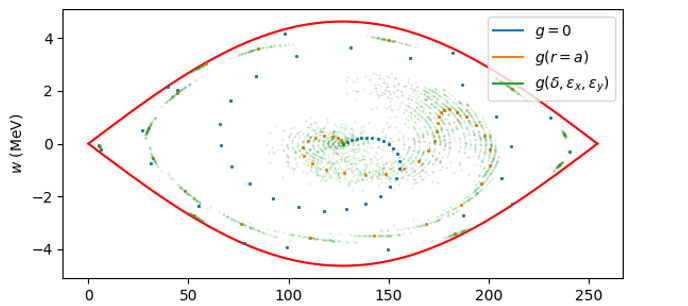
\includegraphics[width=\linewidth]{figs/tune_blurr/trajectories.png}
    \caption{Comparison of Synchrotron motion of ``ghost particles" in a matched longitudinal bunch for single-particle motion, coherent space-charge impedance and incoherent space-charge impedance incorporating betatron motion}
    \label{fig:full_comparison}
\end{figure}

The particles depicted are selected ``ghost" particles visualized within a non-oscillating matched longitudinal bunch. Accordingly, the derivative term related to the longitudinal profile is non-varying as the longitudinal profile is stable. Nonetheless we observe originally the deviation between single-particle motion ($g=0$), coherent space-charge impedance $g(r=a)$ and incoherent space-charge impedance $g(\delta, \epsilon_x, \epsilon_y)$ which approximates betatron motion, further depicted in Figure~\ref{fig:tune_dist_blur}.

\begin{figure}
    \centering
    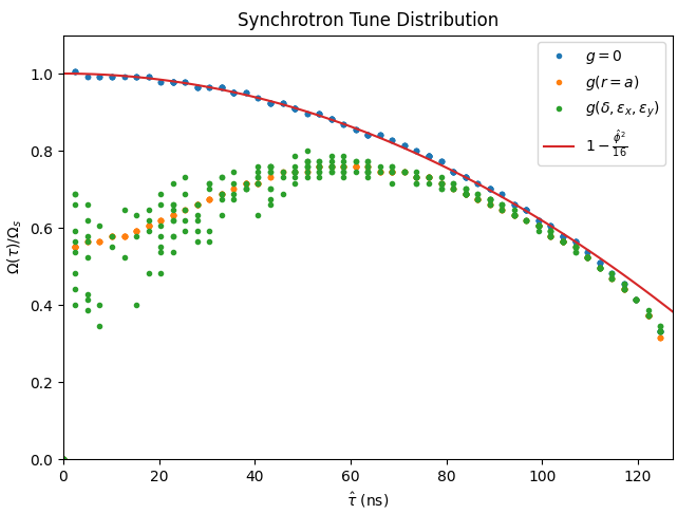
\includegraphics{figs/tune_blurr/normalized_tune.png}
    \caption{Blurring of synchrotron oscillation frequency due to Transverse Motion}
    \label{fig:tune_dist_blur}
\end{figure}

\subsection{Bunch Stability}

A standard \textit{dipole-oscillation} measurement can be used to probe the synchrotron frequency of a given longitudinal bunch distribution. A bunch injected with an offset relative to the synchronous phase will oscillate about the bucket center until it fully filaments, reaching an equilibrium with greater \textit{geometric emittance}, as visible in Figure~\ref{fig:filamentation}.

\begin{figure}
    \centering
    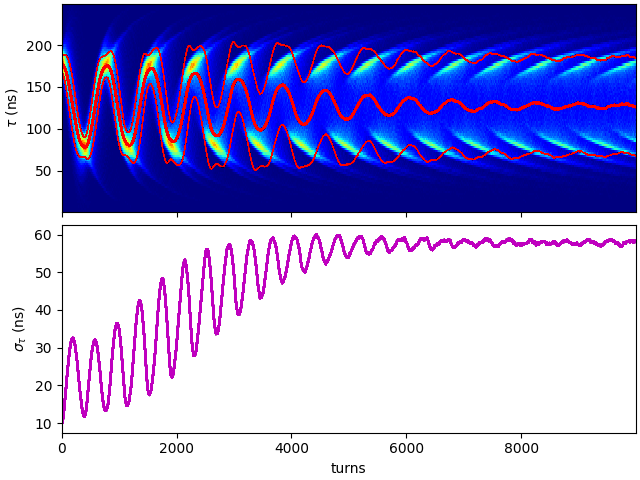
\includegraphics{figs/dipole_oscillation.png}
    \caption{\textbf{BLonD} simulation of dipole oscillations}
    \label{fig:filamentation}
\end{figure}

Tune blurring may increase the observed filamentation rate of our distribution.  Frequently associated as a stabilizing effect, tune spread filamentation will eliminate mismatched bunches or coherent bunch perturbations by distributing these imperfections along Hamiltonian contours. It is therefore reasonable to suspect that the impact of transverse motion on space-charge impedance may provide additional stability to longitudinal motion.

\chapter{Summary and Conclusions}

\section{Experimentation}

Experiments attempting to measure the phenomena of ``tune blurring"  in the PS at \textit{Flat-Bottom} were conducted with the following baseline parameters:

\begin{table}
    \centering
    \begin{tabular}{c|c |c |c}
        parameter  & symbol     & value & unit      \\
        \hline
        harmonic   & h          & 9     &           \\
        voltage    & $V_g$      & 22    & kV        \\
        intensity  & N          & 2e12  & particles \\
        transition & $\gamma_t$ & 6.1   &           \\
    \end{tabular}
    \caption{PS parameters in \textbf{MD} experiments}
    % \label{tab:my_label}
\end{table}

Bunch length and instability measurements can be used to characterize and identify the synchrotron frequency \cite{sacherer_bunch_1977}. A unmatched but centered bunch will contract in accordance with the synchrotron frequency. This generates a \textit{quadrupole-oscillation} of bunch length which can be measured and interpreted to provide insight about the distribution's synchrotron frequency.

\begin{figure}
    \centering
    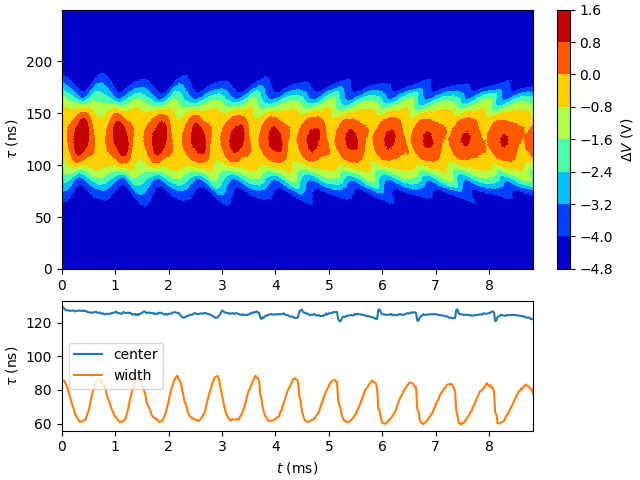
\includegraphics{figs/injosc.14x144.dat.npy.png}
    \caption{Bunch length oscillations from PS intensity experiments}
\end{figure}

In experiment, only the ``bulk" synchrotron frequency can be probed as longitudinal profiles are a 1D projection of a 2D phase-space distribution. Because synchrotron motion with space charge natively yield a tune spread and tune shift,  an effect as subtle as tune ``blur" will be challenging to resolve.

The analysis of these measurements were inconclusive as intrinsic beam instabilities incorporated a high variance between similar measurements. As well, the beam become unstable at higher bunch intensities requiring additional statistics to eliminate outliers. Likely characterizing and quantiying how the ``filamentation rate'' evolves with transverse emittance may provide evidence of this effects existence.

\section{Conclusion}

It has been shown in theory and simulation that the unique motion of a particle's betatron trajectories will provide additional variance to the applied induced voltage due to space-charge impedance. This effect, when captured adequately in longitudinal tracking codes, yields an observed ``blurring" of the synchrotron frequency distribution when compared to that of less sophisticated approaches. The observed ``tune blur" leads to an increased filamentation rate and accordingly may suggest an increase to the dampening rate of longitudinal fluctuations and micro-bunch instabilities. Attempts to measure this filamentation rate variation were unsuccessful however further work may be conducted over a sufficiently long acquisition period so that an oscillating bunch can be observed to fully stabilize and provide greater resolution to the bulk filamentation variation.